%%%%%%%%%%%%%%%%%%%%%%%%%%%%%%%%%%%%%%%%%%%%%%%%%%%%%%%%%%%%%%%%%%%%%%%%%%%%%%%%
%2345678901234567890123456789012345678901234567890123456789012345678901234567890
%        1         2         3         4         5         6         7         8

\documentclass[10pt, conference, compsocconf]{IEEEtran}  % Comment this line out
                                                          % if you need a4paper
%\documentclass[a4paper, 10pt, conference]{ieeeconf}      % Use this line for a4
                                                          % paper

\IEEEoverridecommandlockouts                              % This command is only
                                                          % needed if you want to
                                                          % use the \thanks command
\overrideIEEEmargins
% See the \addtolength command later in the file to balance the column lengths
% on the last page of the document



% The following packages can be found on http:\\www.ctan.org
\usepackage{graphics} % for pdf, bitmapped graphics files
\usepackage{epsfig} % for postscript graphics files
\usepackage{mathptmx} % assumes new font selection scheme installed
\usepackage{times} % assumes new font selection scheme installed
\usepackage{amsmath} % assumes amsmath package installed
\usepackage{amssymb}  % assumes amsmath package installed
\usepackage{xcolor}
\usepackage{subcaption}
\usepackage{todonotes}
\usepackage{tikz}
\usetikzlibrary{positioning}
\usepackage{pgfplots}
\usetikzlibrary{shapes,arrows}

\newtheorem{Theorem}{Theorem}
%\newtheorem{Theorem}{Theorem}[section]
%\numberwithin{Theorem}{section}
\newtheorem{Definition}{Definition}[section]
\numberwithin{Definition}{section}
\newtheorem{Observation}{Observation}
\newtheorem{Claim}{Claim}[section]
\numberwithin{Claim}{section}
% \usepackage{subfigure}
\begin{document}

\title{One Plus One is More than Two: A Practical Combination of Power and Fault Analysis Attacks on PRESENT and PRESENT-like Block Ciphers}

% \author{Blinded for Review}

\author{\IEEEauthorblockN{Sikhar Patranabis, Debdeep Mukhopadhyay}
\IEEEauthorblockA{Department of CSE, IIT Kharagpur, India\\
sikhar.patranabis@iitkgp.ac.in, debdeep@cse.iitkgp.ernet.in}
\and
\IEEEauthorblockN{Jakub Breier, Shivam Bhasin}
\IEEEauthorblockA{Temasek Labs, NTU Singapore\\
% \{JBreier, sbhasin\}@ntu.edu.sg}
jbreier@ntu.edu.sg, sbhasin@ntu.edu.sg}}

% \author{Huibert Kwakernaak$^{1}$ and Pradeep Misra$^{2}$% <-this % stops a space
% \thanks{*This work was not supported by any organization}% <-this % stops a space
% \thanks{$^{1}$H. Kwakernaak is with Faculty of Electrical Engineering, Mathematics and Computer Science,
%         University of Twente, 7500 AE Enschede, The Netherlands
%         {\tt\small h.kwakernaak at papercept.net}}%
% \thanks{$^{2}$P. Misra is with the Department of Electrical Engineering, Wright State University,
%         Dayton, OH 45435, USA
%         {\tt\small p.misra at ieee.org}}%
% }






\maketitle
%\thispagestyle{empty}
%\pagestyle{empty}


%%%%%%%%%%%%%%%%%%%%%%%%%%%%%%%%%%%%%%%%%%%%%%%%%%%%%%%%%%%%%%%%%%%%%%%%%%%%%%%%
\begin{abstract}

We present the first practically realizable side-channel assisted fault attack on PRESENT, that can retrieve the last round key efficiently using single nibble faults. The attack demonstrates how side-channel leakage can allow the adversary to precisely determine the fault mask resulting from a nibble fault injection instance. We first demonstrate the viability of such an attack model via side-channel analysis experiments on top of a laser-based fault injection setup, targeting a PRESENT-80 implementation on an ATmega328P microcontroller. Subsequently, we present a differential fault analysis (DFA) exploiting the knowledge of the output fault mask in the target round to recover multiple last round key nibbles independently and in parallel. Both analytically and through experimental evidence, we show that the combined attack can recover the last round key of PRESENT with 4 random nibble fault injections in the best case, and around 7-8 nibble fault injections in the average case. Our attack sheds light on a hitherto unexplored vulnerability of PRESENT and PRESENT-like block ciphers that use bit-permutations instead of maximum distance separable (MDS) layers for diffusion.
\end{abstract}




\begin{IEEEkeywords}
DFA, DPA, PRESENT, combined attacks, fault attacks, side-channel analysis, bit-permutation
% component; formatting; style; styling;

\end{IEEEkeywords}
\IEEEpeerreviewmaketitle


%%%%%%%%%%%%%%%%%%%%%%%%%%%%%%%%%%%%%%%%%%%%%%%%%%%%%%%%%%%%%%%%%%%%%%%%%%%%%%%%
\section{INTRODUCTION}


The advent of pervasive devices for communication and information systems such as the Internet of Things (IoT) has led to an increased demand for embedded security solutions with a good balance of performance and security. In particular, IoT applications have motivated a whole branch of cryptographic design, denoted as \emph{lightweight cryptography}. The aim of lightweight cryptography is to design security primitives, such as block ciphers, that have low area footprint, reasonable throughput, low energy consumption, and provide adequate security guarantees against classical cryptanalytic attacks. While design and analysis of block ciphers requires careful consideration, real-world security also mandates secure implementations for the same. In particular, such implementations must resist side-channel attacks (SCA) as well as fault attacks (FA). %It is expected that in the near future, lightweight block ciphers such as PRESENT form crucial building blocks in the design of secure embedded devices for IoT and for the cyber-physical space in general.

One of the most popular lightweight block ciphers is PRESENT \cite{DBLP:conf/ches/BogdanovKLPPRSV07}. % which uses a substitution-permutation network (SPN) spread across 31 rounds, and affords 80/128 bit-security for a plaintext block of size 64.
The design of PRESENT has inspired a whole new family of block ciphers that use bit-permutations as opposed to maximum distance separable (MDS) layers for achieving the necessary diffusion characteristics. Bit-permutations have zero-cost implementation in hardware as they can be realized solely via wiring. Several new proposals for lightweight block ciphers such as Rectangle \cite{DBLP:journals/chinaf/ZhangBLR0V15} and GIFT \cite{gift} have opted for bit-permutations for efficiency in hardware. In this paper, we propose a novel side-channel assisted fault analysis of PRESENT and PRESENT-like ciphers that exposes an interesting vulnerability of bit-permutations. In particular, the attack is based on the principle that for bit-permutation based ciphers, the knowledge of the output fault mask in an earlier round could be exploited to significantly reduce the entropy of the input fault mask at a later round. 



 %SCAs exploit the leakage from a target device executing a cryptographic algorithm to try and retrieve the secret key using divide and conquer techniques. There exist today extremely strong passive SCAs such as the differential power analysis (DPA) that exploits the correlation between physical measurements such as power dissipation obtained at various time instances, and the internal state of the processing device at those time instances, to reveal the secret key. In active side-channel attacks, such as differential fault analysis (DFA), an adversary injects faults to disturb the normal execution of cryptographic systems, and then analyzes the corresponding leakage behavior to try and retrieve the secret key. SCA and FA are potent threats to cryptographic implementations since they are practical to mount, require low cost equipment, and render even mathematically robust and cryptographically secure algorithms vulnerable. Fault attacks such as the Row-Hammer attacks \cite{} can even be mounted remotely using a simple JavaScript browser \cite{}. Such attacks are particularly relevant in the context of IoT, where hundreds of devices running secure applications are either physically or remotely accessible to adversaries.

The main contributions of this paper are as follows:

\begin{enumerate}
\item The paper proposes the first practically realizable combination of side-channel analysis (SCA) and differential fault analysis (DFA) on PRESENT. The attack uses a relaxed fault model corresponding to a given target round, and assumes that the adversary uses side-channel leakage to precisely determine the resulting fault mask. Prior attacks on PRESENT have mostly been limited to either SCA or FA, but have not exploited the combined potential of both. We present a theoretical analysis to establish that the attack is capable of recovering multiple key nibbles in parallel under the same fault injection instance, implying that the attack is not only feasible but also efficient.

\item We corroborate the theoretical analysis with a real-world demonstration of the combined attack on an ATmega328P microcontroller-based implementation of PRESENT-80 using a laser-driven fault injection setup. Our experiments demonstrate that the proposed attack recovers 64 bits of the last round key of PRESENT using only 4 fault injections in the best case, and 7-8 fault injections in the average case. This makes our attack one of the most efficient to be proposed on PRESENT and PRESENT-like block ciphers.

\end{enumerate}

% \subsection{Bit-permutations: Inherently weak against combined attacks?}

% Our combined attack is, in principle, aided by the diffusion characteristics of PRESENT. This sheds light on an hitherto unexploited weakness of bit-permutations: the knowledge of the output mask of a suitable injected fault in an earlier round can be used to significantly reduce the entropy of the output fault mask in a subsequent round, even if the two rounds are executed as many as three clock cycles apart. The same attack would not, however, apply to an MDS-layer based block cipher such as AES, where such fault propagation characteristics are absent. To the best of our knowledge, our work is the first to demonstrate this inherent vulnerability of PRESENT and PRESENT-like block ciphers using bit-permutations for implementation efficiency. 


\section{Preliminaries}

\subsection{Overview of the PRESENT Block Cipher}

% \begin{figure}
%   \begin{center}
%  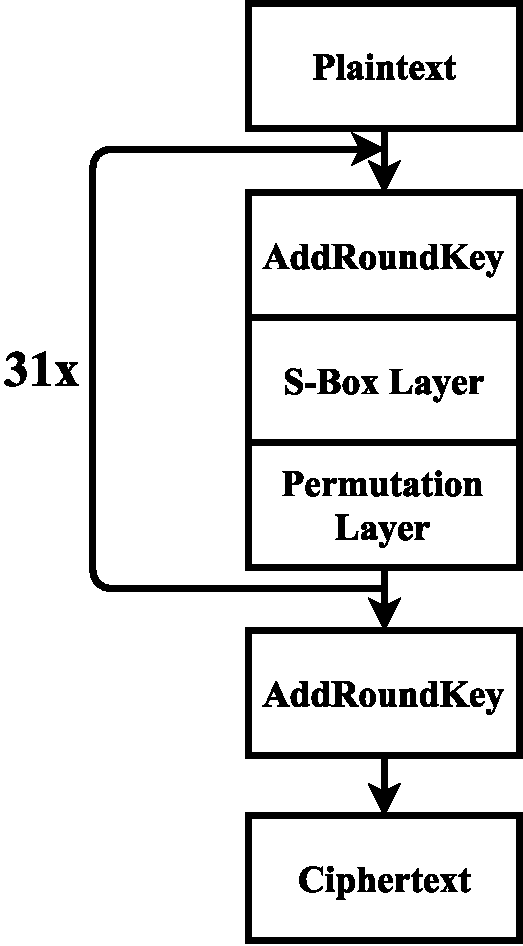
\includegraphics[scale=0.25]{PRESENT.pdf} 
%  \caption{\scriptsize{An Overview of PRESENT}}
%  \label{fig:overview}
%  \end{center}
% \end{figure}
% \todo[inline]{Figure can be compressed}

\begin{table}
\centering
\caption{The PRESENT S-Box}
\label{tab:PRESENT-S-Box}
% \caption{The PRESENT Block Cipher}
% \label{tab:PRESENT}
% \begin{subtable}{.5\textwidth}
% \centering
\scalebox{0.7}{
\begin{tabular}{|c||c|c|c|c|c|c|c|c|c|c|c|c|c|c|c|c|}
\hline
& & & & & & & & & & & & & & & &\\
$x$ & 0 & 1 & 2 & 3 & 4 & 5 & 6 & 7 & 8 & 9 & A & B & C & D & E & F\\
& & & & & & & & & & & & & & & &\\\hline
& & & & & & & & & & & & & & & &\\
$S\left[x\right]$ & C & 5 & 6 & B & 9 & 0 & A & D & 3 & E & F & 8 & 4 & 7 & 1 & 2\\
& & & & & & & & & & & & & & & &\\\hline
% Chakraborty et al.~\cite{chakrabortycombined} & 2015 & Grainv1 & DPA + Bit-flip Fault\\\hline
\end{tabular}}
\end{table}

\begin{figure}
	\centering
	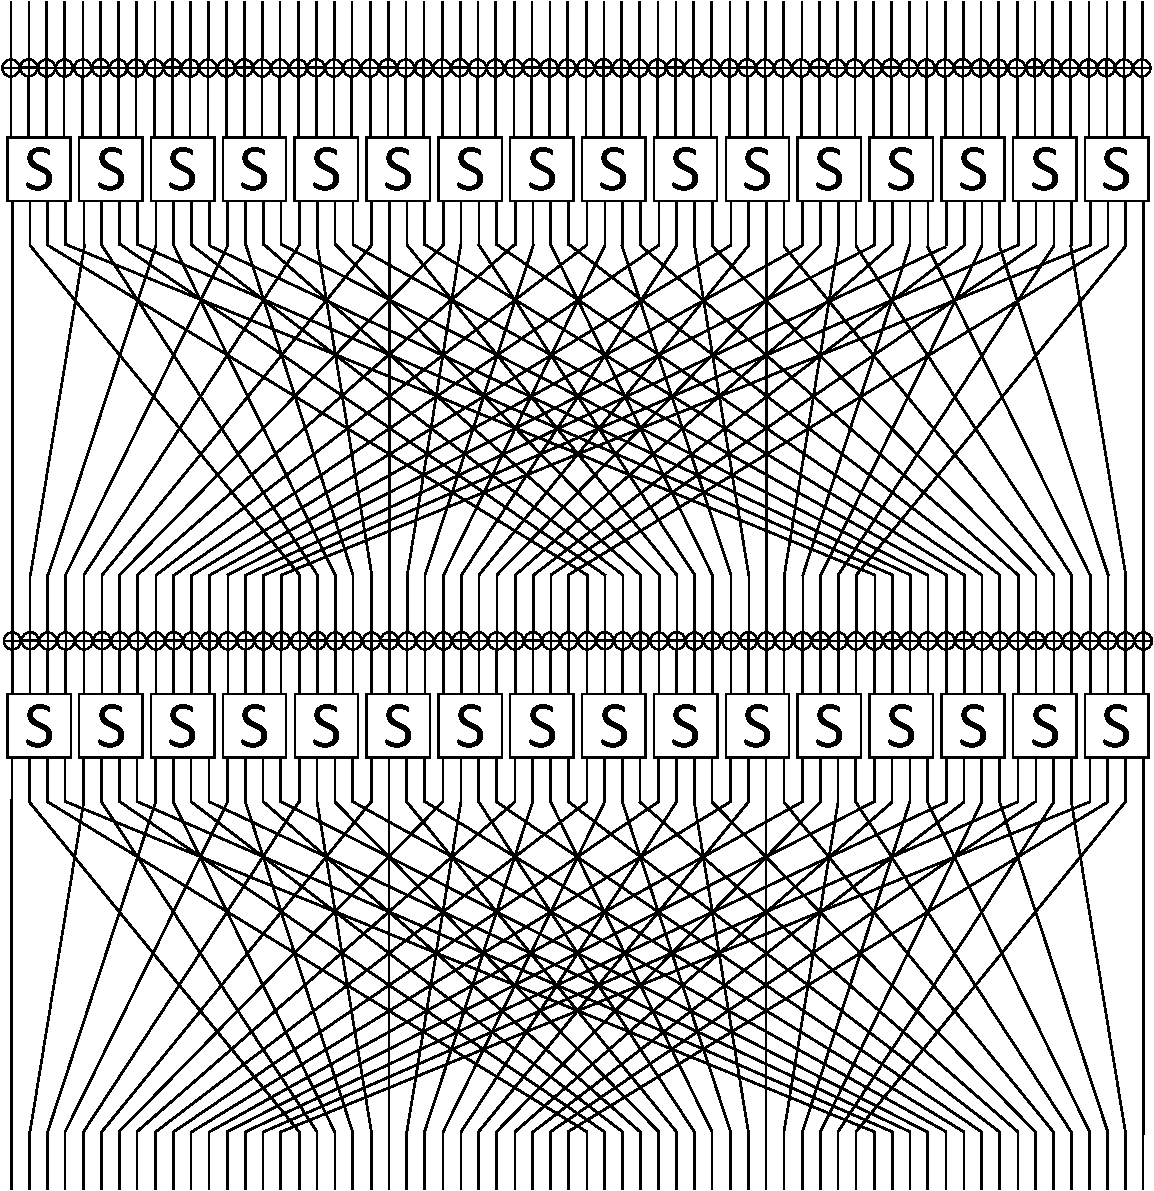
\includegraphics[scale=0.3]{present_structure}
    \caption{Structure of two rounds of PRESENT}
    \label{fig:present_structure}
\end{figure}

% \begin{table}
% \caption{The PRESENT bit-permutation Layer}
% \label{tab:PRESENT-Perm}
% % \begin{subtable}{.5\textwidth}
% % \captionsetup{font=scriptize}
% \centering
% \scalebox{0.7}{
% \begin{tabular}{|c||c|c|c|c|c|c|c|c|c|c|c|c|c|c|c|c|}
% \hline
% & & & & & & & & & & & & & & & &\\
% $i$ & 0 & 1 & 2 & 3 & 4 & 5 & 6 & 7 & 8 & 9 & 10 & 11 & 12 & 13 & 14 & 15\\
% & & & & & & & & & & & & & & & &\\
% $P(i)$ & 0 & 16 & 32 & 48 & 1 & 17 & 33 & 49 & 2 & 18 & 34 & 50 & 3 & 19 & 35 & 51\\\hline\hline
% & & & & & & & & & & & & & & & &\\
% $i$ & 16 & 17 & 18 & 19 & 20 & 21 & 22 & 23 & 24 & 25 & 26 & 27 & 28 & 29 & 30 & 31\\
% & & & & & & & & & & & & & & & &\\
% $P(i)$ & 4 & 20 & 36 & 52 & 5 & 21 & 37 & 53 & 6 & 22 & 38 & 54 & 7 & 23 & 39 & 55\\\hline\hline
% & & & & & & & & & & & & & & & &\\
% $i$ & 32 & 33 & 34 & 35 & 36 & 37 & 38 & 39 & 40 & 41 & 42 & 43 & 44 & 45 & 46 & 47\\
% & & & & & & & & & & & & & & & &\\
% $P(i)$ & 8 & 24 & 40 & 56 & 9 & 25 & 41 & 57 & 10 & 26 & 42 & 58 & 11 & 27 & 43 & 59\\\hline\hline
% & & & & & & & & & & & & & & & &\\
% $i$ & 48 & 49 & 50 & 51 & 52 & 53 & 54 & 55 & 56 & 57 & 58 & 59 & 60 & 61 & 62 & 63\\
% & & & & & & & & & & & & & & & &\\
% $P(i)$ & 12 & 28 & 44 & 60 & 13 & 29 & 45 & 61 & 14 & 30 & 46 & 62 & 15 & 31 & 47 & 63\\\hline
% \end{tabular}}
% % \end{subtable}
% \end{table}

% \todo[inline]{The attack is on PRESENT. 80 and 128 only applies to key schedule and thus no difference for the attack.}
%We present a brief overview of our target block cipher - PRESENT-80.
PRESENT  is based  on a substitution-permutation network (SPN).  It  consists  of 31 rounds, block length is 64 bits and it supports keys with lengths of 80 and 128 bits. In this paper, we focus on the 80 bit key length version, which we denote as PRESENT-80, however the attack applies on 128-bit as well. %(note that this is also the version recommended by the designers of PRESENT).
Each  round  consists  of  three operation layers: an XOR-layer with  the  round key, a substitution layer using $16$ identical $4\times 4$ S-Box (Table \ref{tab:PRESENT-S-Box}) and a bit-permutation layer (Figure \ref{fig:present_structure}). At the end of round 31, a post-whitening XOR with the round key is performed, so 32  round  keys are generated in total. The key schedule for PRESENT-80 comprises of a rotation, S-Box look-up and round counter addition, thus making it invertible.


%Key schedule of PRESENT-80 is as follows: Let the original secret key stored in the register be $K=k_{79}k_{78}\cdots k_{0}$. Each round key $K_i$ for $1\leq i \leq 32$ uses the 64 leftmost bits $k_{79}k_{78}\cdots k_{16}$ of the key register at that point. After every round, the key register $K$ is updated as follows:
%\begin{itemize}
%\item $\left[k_{79}k_{78}\cdots k_{1}k_{0}\right] = \left[k_{18}k_{17}\cdots k_{1}k_{0}k_{79}k_{78}\cdots k_{20}k_{19}\right]$
%\item $\left[k_{79}k_{78}k_{77}k_{76}\right] = S\left[k_{79}k_{78}k_{77}k_{76}\right]$
%\item $\left[k_{19}k_{18}k_{17}k_{16}k_{15}\right] = \left[k_{19}k_{18}k_{17}k_{16}k_{15}\right] \oplus \text{\textsf{RC}}$
%\end{itemize}
%\noindent where $\text{\textsf{RC}}$ is a round counter.

% \begin{figure}
%   \begin{center}
%  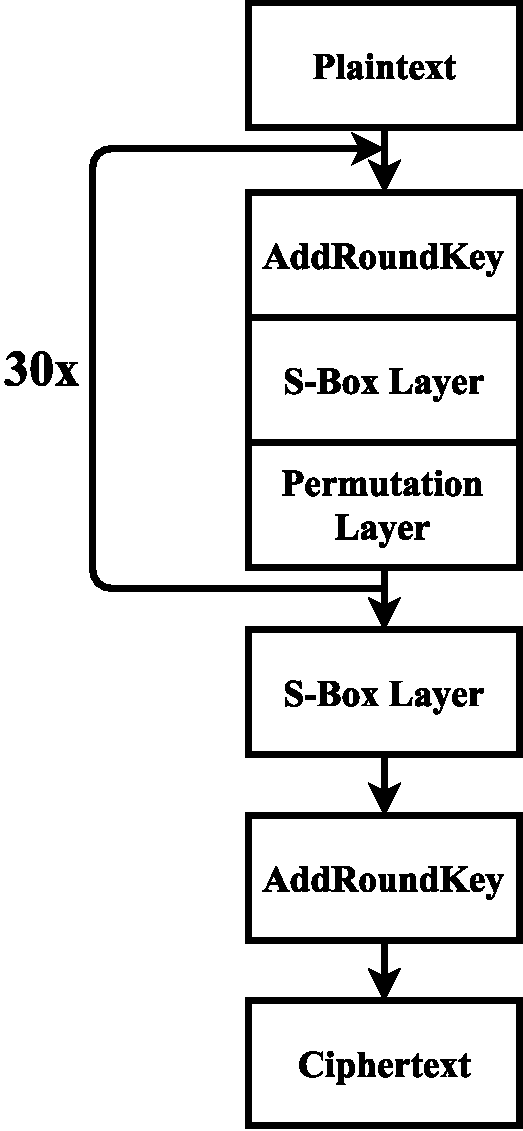
\includegraphics[scale=0.2]{PRESENT_Reduced.pdf} 
%  \caption{\scriptsize{A Modified PRESENT}}
%  \label{fig:PRESENT_mod}
%  \end{center}
% \end{figure}
% \todo[inline]{If space is an issue, this figure might be removed}


\subsection{Related Work}

% \subsubsection{Combined SCA and FA on Symmetric-Key Cryptosystems}

% While both SCA and FA are powerful attacks on their own, some works have explored the combined power of the two.%recent literature has also explored means to enhance attack potency via a combination of these attach techniques. Traditionally SCA has been viewed as employing non-invasive techniques such as power detection, while FA is expected to be the semi-invasive/invasive counterpart in implementation attacks. 
% The first such combined attack was proposed by Skorobogatov~\cite{skorobogatov2006optically}, where he used a laser beam to illuminate a specific area on the chip surface, thereby enhancing its observability for side-channel attacks. It was demonstrated on the SRAM of a PIC microcontroller, and allowed access to individual bits as opposed to using the more traditional Hamming weight model. %Although this technique is hard to apply on sub-micron technology with multiple metal layers, it represents the first ever attempt at combining SCA with semi-invasive attacks. Subsequently, a number of such combined attacks have been proposed on both public-key and symmetric-key cryptosystems, which we briefly review here.

% % \subsubsection{Combined SCA and FA on Public-Key Cryptosystems}

% % \begin{table*}[t]
% % \centering
% % \caption{Summary of Combined SCA and FA on PKC}
% % \label{tab:pkc}
% % \begin{tabular}{|c|c|c|c|}
% % \hline
% % Reference & Year &  Target & Combination\\\hline\hline
% % Amiel et al~\cite{amiel2007passive} & 2007 & Atomic left-to-right exponentiation & SPA + Instruction Skip Fault\\\hline
% % Schmidt et al~\cite{schmidt2010combined} & 2010 & Atomic left-to-right exponentiation & SPA + Instruction Skip Fault\\\hline
% % Fan et al.~\cite{fan2011infinity} & 2011 & Scalar multiplication & SPA + Bit-flip Fault\\\hline
% % Vuillaume et al.~\cite{vuillaume2012rsa} & 2012 & Prime generation & DPA + Template + Instruction Skip Fault\\\hline 
% % Feix et al~\cite{feix2013defeating} & 2013 & Atomic left-to-right exponentiation & DPA/Template + Instruction Skip Fault\\\hline
% % Barbu et al.~\cite{barbu2013combined} & 2013 & RSA-CRT & DPA + Stuck-At Fault\\\hline
% % Kim et al.~\cite{kim2013new} & 2013 & BNP exponentiation & SPA + Instruction Skip Fault\\\hline
% % Su et al.~\cite{su2015combined} & 2015 & Bocher exponentiation & SPA + Instruction Skip Fault\\\hline
% % \end{tabular}
% % \end{table*}

% % A summary of state-of-the art combined SCA and FA attacks on public-key cryptosystems is presented in Table \ref{tab:pkc}. The first practical combined SCA and FA was performed on RSA by Amiel et al~\cite{amiel2007passive}. It was able to recover the secret key with only one side-channel trace from a simple power analysis (SPA) resistant RSA implementation. The fault was used to skip register initialization at the beginning of exponentiation, which leads to SPA leakage and secret retrieval. Even if the implementation detects the fault and did not return the signature, the exponent can already be extracted. This attack methodology was generalized and extended in the context of ECC by Schmidt et al. in~\cite{schmidt2010combined}. Schmidt et al. also proposed a combined attack resistant exponentiation to counter this attack. This countermeasure was shown to be vulnerable to combined attacks and was further improved in~\cite{feix2013defeating}. A similar attack and improvement on BNP exponentiation and application to CRT-RSA was proposed by Kim et al.~\cite{kim2013new}. The attack of~\cite{amiel2007passive} was also shown practical for Bocher's exponentiation~\cite{boscher2009blinded} by Su et al. in~\cite{su2015combined}.  

% A combined attack technique targeting the scalar multiplication of ECC was proposed in~\cite{fan2011infinity}. The attack exploited special input points whose order can be highly reduced using fault injection. In particular, the points when at infinity leak on the SCA signature of the multiplication, and from it, the secret key. A set of attacks on prime generation for public key cryptography is proposed in~\cite{vuillaume2012rsa}. The attack combines a differential power analysis (DPA) attack, a template attack and a fault attack. The DPA attack reveals a few of the least significant bits of prime candidates, while the template attack targets  the most significant bits. The fault attack is used to prevent quick termination of prime search operation, thus allowing higher number of samples for power analysis. In~\cite{barbu2013combined}, Barbu et al. propose a combined attack on CRT-RSA implementation protected with blinding countermeasures and verifies signature using public exponent. They demonstrate that a fault during the signature computation, and SCA on the signature verification can reveal sensitive information to the attacker.
% This information can then be used to factorize the whole public modulus and thus retrieve the secret key. 

%\subsection{Combined SCA and FA on Symmetric-Key Cryptosystems}

\begin{table}[t]
\centering
\caption{Summary of Combined SCA and FA on Block Ciphers}
\label{tab:skc}
\scalebox{0.75}{
\begin{tabular}{|c|c|c|c|}
\hline
Reference & Setting &  Target & Combination\\\hline\hline
Robisson et al~\cite{robisson2007differential} & Simulated & Non-masked AES & DPA + Stuck-At\\\hline
Clavier et al.~\cite{clavier2010passive} & Simulated & Masked AES & CPA + Instruction-skip\\\hline
Roche et al.~\cite{roche2011combined} & Simulated & Key Schedule of Masked AES & CPA + Stuck-At or Byte\\\hline
Dassance et al.~\cite{dassance2012combined} & Simulated & Key Schedule of Masked AES & CPA + Byte\\\hline
Moradi et al.~\cite{moradi2011power} & Practical & Unprotected + Protected AES & CCA + FSA\\\hline
Li et al.~\cite{li2013exploring} & Practical & Unprotected AES & DPA + FSA \\\hline
% Chakraborty et al.~\cite{chakrabortycombined} & 2015 & Grainv1 & DPA + Bit-flip Fault\\\hline
\end{tabular}}
\end{table}
%A summary of state-of-the art combined SCA and FA attacks on block ciphers is presented in Table \ref{tab:pkc}. The foremost instance of combined SCA and FA on block ciphers is 
% Differential behavioral analysis (DBA ~\cite{robisson2007differential}) combined SCA with safe-error attacks. Assuming stack-at fault model it observes if fault alters the side-channel behavior of the computation to derive the key.  A combined SCA and FA on AES was proposed in~\cite{clavier2010passive}. It targets the first key addition in AES and based on instruction-skip/change fault model to preferably force XOR output to 0. Under this fault model, the ciphertext is compared with original ciphertext, and the XOR output is inferred to be 1 or 0 depending on whether the ciphertext changes or not. The attack was further enhanced using correlation power analysis (CPA) to break a masked AES implementation. Roche et al. proposed a DFA on AES key schedule in~\cite{roche2011combined} by injecting faults in pen-ultimate round key computation. They further extend this attack to a combined setting, where SCA measurements are used to aid DFA on the key schedule of a masked AES. This attack was subsequently improved in~\cite{dassance2012combined}, where the authors reduce the strict restrictions on fault repeatability, model and location, that were imposed by the original attack. All these attack were demonstrated in simulated settings. A different family of fault attack i.e. fault sensitivity analysis (FSA) was also combined with side-channel. Moradi et al. ~\cite{moradi2011power} combined collision correlation attack (CCA) and FSA. The combined attack exploits either non-uniform fault distribution or data-dependent timing of faults, and was successfully demonstrated on several unprotected and protected AES cores on SASEBO LSI chips. In another work~\cite{li2013exploring}, the authors use FSA to develop a leakage model which is then used to launch a power based key recovery attack. Both these attacks were demonstrated with real measurements. To the best our knowledge, no previous work demonstrates a practical attack combining DFA with side-channel.

% \subsubsection{DFA on PRESENT}
The first DFA on PRESENT, published by G. Wang and S. Wang~\cite{present_dfa1} required 64 pairs of correct and faulty ciphertext on average, with a computational complexity of $2^{29}$. Later, Zhao et al.~\cite{present_dfa2} utilized a fault-propagation pattern-based DFA, targeting PRESENT and PRINT. The attack on PRESENT-80/128 required 8/16 ciphertext pairs on average, reducing the key search space to $2^{14.7}/2^{21.1}$ in average. Bagheri et al.~\cite{present_dfa3} showed attacks utilizing single bit-flip and single nibble fault models. The first attack obtains the last subkey with 48 ciphertexts pairs, while the second attack reveals the key with 18 ciphertext pairs on average. Breier and He~\cite{siot2015} proposed a multiple fault attack, targeting four nibbles at once, being able to recover the secret key in 2 encryptions.
DeSantis et al.~\cite{DeSantis2015} presented a ciphertext-only attack, which requires only two ciphertext pairs in the best case. Ghalaty et al.~\cite{Ghalaty2015} attacked PRESENT and LED ciphers with Differential Fault Intensity Analysis (DFIA), showing that both ciphers can be broken with a practically feasible number of fault injections. 

A summary of state-of-the art combined SCA and FA attacks on block ciphers is presented in Table \ref{tab:skc}.
Differential behavioral analysis (DBA ~\cite{robisson2007differential}) is a combined SCA with safe-error attacks.
A combined SCA and FA targeting first AES key addition was proposed in~\cite{clavier2010passive}.
Roche et al. proposed a DFA on AES key schedule in~\cite{roche2011combined} by injecting faults in pen-ultimate round key computation, further improved in~\cite{dassance2012combined}.
All these attack were demonstrated in simulated settings.
Combinations of fault sensitivity analysis (FSA) with collision correlation attack (CCA)~\cite{moradi2011power} and CPA were also proposed.~\cite{li2013exploring}.
%These include differential behavioral analysis (DBA ~\cite{robisson2007differential}), fault and side channel (~\cite{roche2011combined}) and combinations of collision correlation attack (CCA) with fault sensitivity analysis (FSA)~\cite{moradi2011power}.
To the best of ours knowledge, no previous work demonstrates a practical demonstration of combining DFA with SCA on PRESENT.

\section{The Proposed Combined SCA and DFA of PRESENT}

In this section, we propose a combined SCA and DFA of PRESENT. We now present a detailed description of the fault attack.

\subsection{Properties of the PRESENT Block Cipher}
\label{subsec:properties}

We begin with a description of the properties of PRESENT that are exploited in our attack. We would like to point out that these properties are due to the bit-permutation layer of PRESENT, and are also observed in other PRESENT-like block ciphers that use bit-permutations as opposed to MDS layers for diffusion.

\begin{itemize}
\item The input of an S-Box in round $r$ comprises output bits from four different S-Boxes in round $r-1$.
\item The output of an S-Box in round $r$ is distributed across the inputs of four different S-Boxes in round $r+1$.
% \item The distribution of inputs and outputs across consecutive rounds occurs among four distinct groups of S-Boxes:
% \begin{itemize}
% \item The output of S-Boxes $0-3$ in round $r$ constitute the inputs for the S-Boxes $0,4,8$ and $12$ in round $r+1$.
% \item The output of S-Boxes $4-7$ in round $r$ constitute the inputs for the S-Boxes $1,5,9$ and $13$ in round $r+1$.
% \item The output of S-Boxes $8-11$ in round $r$ constitute the inputs for the S-Boxes $2,6,10$ and $14$ in round $r+1$.
% \item The output of S-Boxes $12-15$ in round $r$ constitute the inputs for the S-Boxes $3,7,11$ and $15$ in round $r+1$.
% \end{itemize}
\item The output of the S-Box group $[4n,4n+3]$ in round $r$ entirely constitutes the input for the S-Box group $\{n, n+4,n+8, n+12\}$ in round $r+1$, where $n\in\{0,1,2,3\}$. More precisely, for $n,d,l\in\{0,1,2,3\}$, the $l^{\text{th}}$ bit in the output of S-Box $4n+d$ in any round is precisely the $d^{\text{th}}$ bit in the input of S-Box $n+4l$ in the next round, albeit after XOR-ing with the corresponding round key bit. As stated before, visualization of this propagation is depicted in Figure~\ref{fig:present_structure}.
\end{itemize}


\subsection{Fault Model and Fault Location}

Our attack assumes random nibble fault model. The fault is injected at the input of round 28 during a PRESENT encryption operation. Nibble faults have been demonstrated to be practically achievable using traditional fault injection techniques such as clock and voltage glitches \cite{Agoyan:0,Barenghi2} as well as more advanced injections methods such as electromagnetic (EM) pulse or laser pulse injection \cite{Dehbaoui,Trichina}. We use the term \emph{output fault mask} to denote the differential $\Delta_{\text{out}}$ of the correct and faulty nibble at output of S-Box operation in round 28. We would like to point out that recent attacks on PRESENT, such as that presented by Breier et al. in \cite{siot2015}, assume some specific instances of nibble faults that result in a desired output fault mask. Our attack, on the other hand, assumes a random nibble fault, without any specific requirements on the nature of the corresponding output fault mask. This makes our fault model more relevant in the context of real-world fault attacks.

\subsection{The Role of Side-Channel Analysis in Our Attack}
\label{subsec:SCA}

The role of the side-channel leakage in our analysis is to deterministically obtain the output fault mask $\Delta_{\text{out}}$ corresponding to round 28. Note that since our attack assumes a random fault in a single nibble, the output fault mask $\Delta_{\text{out}}$ is not known. Instead, we use side-channel analysis to determine $\Delta_{\text{out}}$. The basic principle is as follows: assuming the fault is injected in a particular nibble during round $r$ (round 28 in our attack on PRESENT), we collect the leakage traces corresponding to the fault-free and faulty computations in round $r+1$ (round 29 in our attack). By computing the difference in side-channel measurements of correct and faulty execution, the bit-permutation pattern makes it possible to determine the exact value of $\Delta_{\text{out}}$. 
We practically demonstrate the recovery of $\Delta_{\text{out}}$, when injecting faults using a laser fault injection a 8-bit micro-controller platform. %(see Section \ref{sec:results} for more details on the experimental set-up).
The fault was injected during the S-Box lookup corresponding to the target nibble in round 28 of PRESENT encryption. %The fault mask  $\Delta_{\text{out}}$ is thus the $x\oplus S[x]$, where x is the nibble value prior to the S-Box operation. 
The fault injection timings were profiled with respect to each nibble operation, allowing a $100\%$ repeatability in corrupting a target nibble. %This validates our assumption that the fault location is precisely known to the adversary during the SCA.
This was followed by a differential analysis between the leakage traces corresponding to the fault-free and faulty computations to retrieve the output fault mask. Detailed experimental results corresponding to the SCA are presented in Section \ref{sec:results}.

\subsection{The Fault Propagation Characteristics}
\label{subsec:propagation}

We now present the fault propagation characteristics corresponding to our attack in details. As already mentioned, the attack targets a single nibble in round 28 of PRESENT. We begin by stating the following theorems.

\begin{Theorem}
\label{th:HW}
Suppose the Hamming Weight of the output fault mask of the target nibble in round $28$ of PRESENT is $x$, where $x\in\{0,1,\cdots,4\}$. Then, the Hamming Weight of the input fault mask of any nibble in round $31$ is at most $x$.
\end{Theorem}
\begin{Theorem}
\label{th:Val}
Suppose the Hamming Weight of the output fault mask of the target nibble in round $28$ of PRESENT is $x$, where $x\in\{0,1,\cdots,4\}$. Then, the input fault mask of any nibble in round $31$ takes at most $2^x$ values.\\
\end{Theorem}

\noindent We first present a concrete example to support the above theorems, and then prove them for generalized instances.
% \begin{itemize}
\subsubsection{\textbf{A Concrete Example}} Suppose the output fault mask of the target nibble in round $28$ of PRESENT is $0001$. This implies that in round $29$, nibble 0 has an input fault mask of $0001$. Unfortunately, the corresponding output fault mask is non-deterministic: all one can infer is that each of the nibbles 0, 4, 8 and 12 in round 30 have an input fault mask of 0000 (implying no fault propagation) or 0001 (implying fault propagation). Once again, the output fault masks in round 30 are non-deterministic; however, one can easily make the following observations:
\begin{itemize}
\item If the input fault mask for nibble 0 in round 30 is 0001, then the input fault mask for nibbles 0, 4, 8 and 12 in round 31 are either 0000 or 0001. On the other hand, if the input fault mask for nibble 0 in round 30 is 0000, then the input fault mask for nibbles 0, 4, 8 and 12 in round 31 is definitely 0000.

\item If the input fault mask for nibble 4 in round 30 is 0001, then the input fault mask for nibbles 1, 5, 9 and 13 in round 31 are either 0000 or 0001. The case of input fault mask 0000 follows analogously.

\item If the input fault mask for nibble 8 in round 30 is 0001, then the input fault mask for nibbles 2, 6, 10 and 14 in round 31 are either 0000 or 0001. The case of input fault mask 0000 follows analogously.  

\item Finally, if the input fault mask for nibble 12 in round 30 is 0001, then the input fault mask for nibbles 3, 7, 11 and 15 in round 31 are either 0000 or 0001. The case of input fault mask 0000 follows analogously. 
\end{itemize}
\noindent Thus, for each of the nibbles in round 31, the input fault mask is either 0000 or 0001, and has Hamming weight at most 1. Figure \ref{example_1} illustrates the fault propagation characteristics for the above example.\\
\begin{figure}
	\centering
	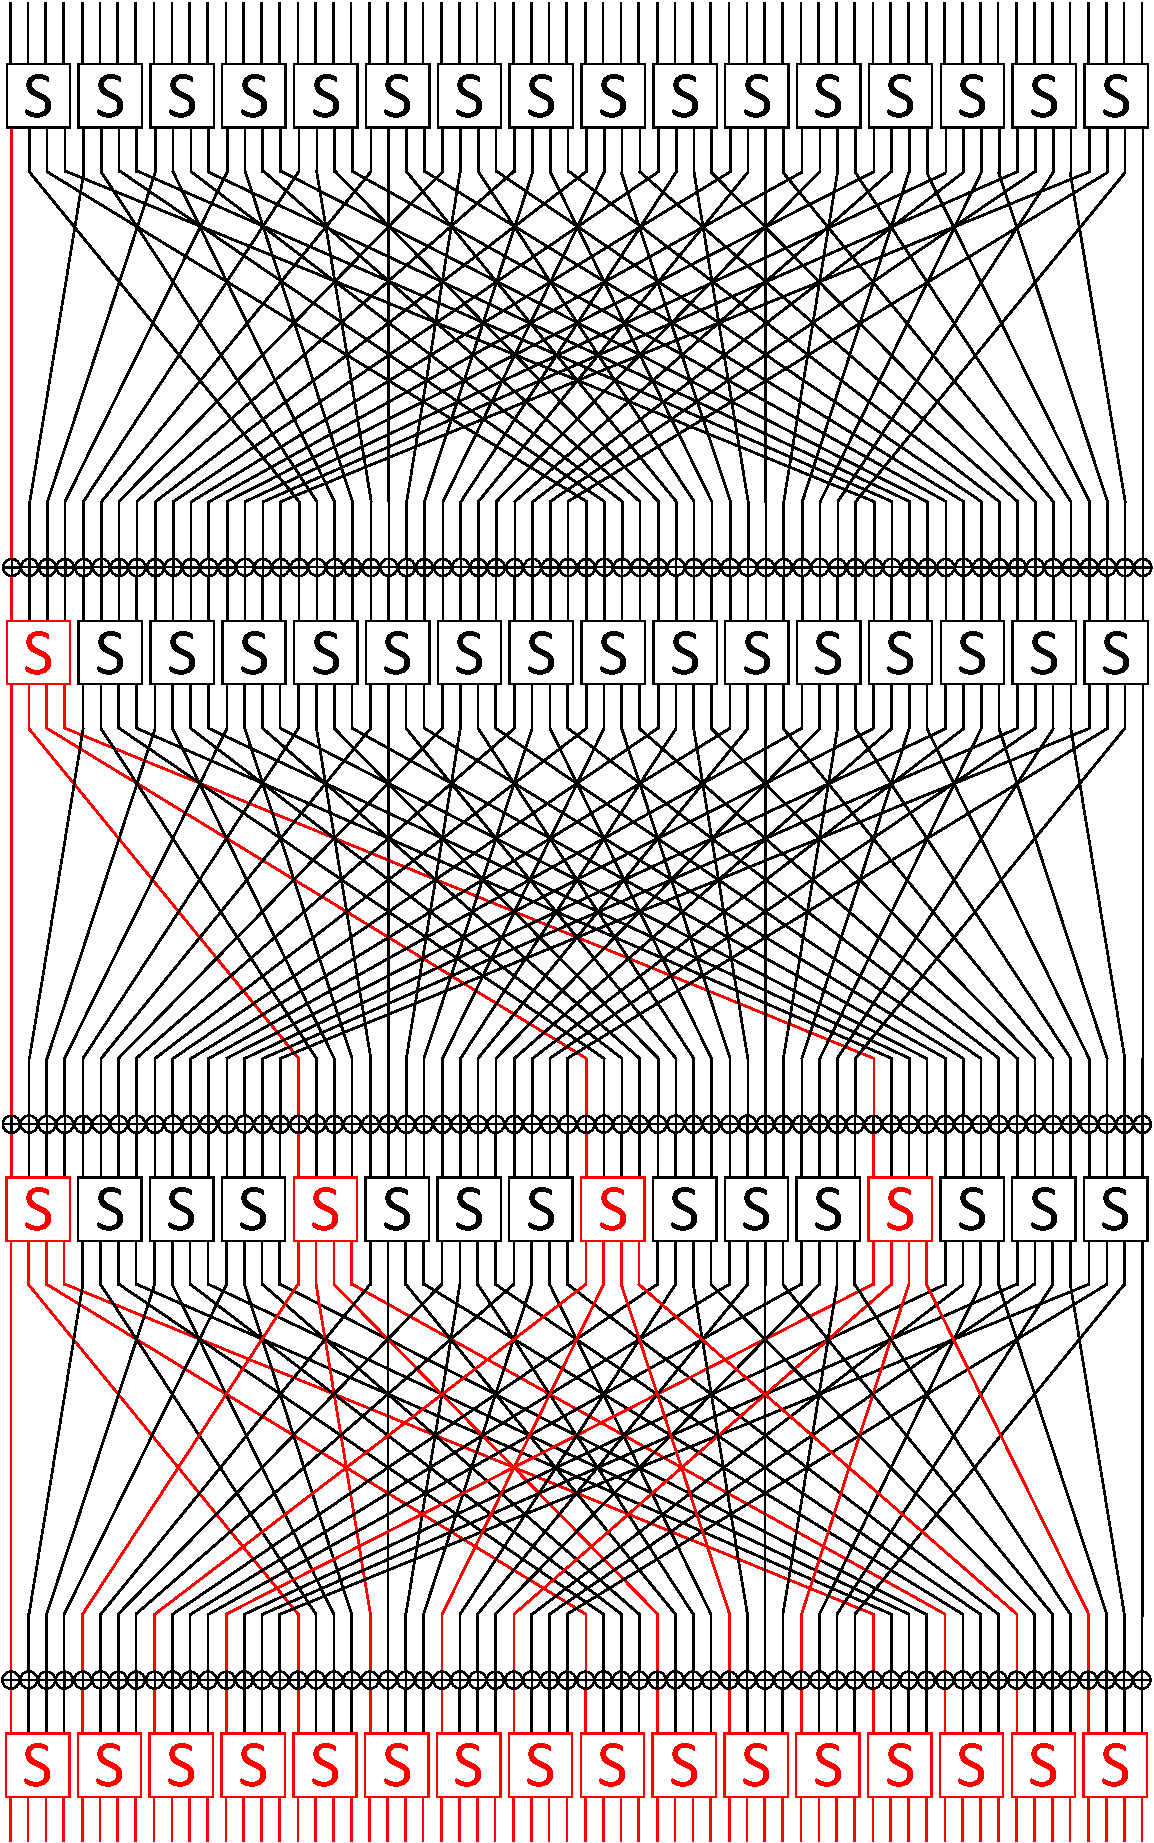
\includegraphics[width=0.9\linewidth]{present_fault_0001}
    \caption{Fault propagation for the output fault mask $0001$}
    \label{example_1}
\end{figure}

% \subsubsection{\textbf{A Concrete Example}} Suppose the output fault mask of the target nibble in round $28$ of PRESENT is $0011$. This implies that in round $29$, nibble 0 and nibble 4 has an input fault mask of $0001$. We can further infer the following (see Figure \ref{example_2} for an illustration):
% \begin{itemize}
% \item Each of the nibbles 0, 4, 8 and 12 in round 30 have an input fault mask of 0000 (implying no fault propagation) or 0001 (implying fault propagation).
% \item Similarly, each of the nibbles 1, 5, 9 and 13 in round 30 have an input fault mask of 0000 (implying no fault propagation) or 0001 (implying fault propagation).
% \end{itemize}
% \noindent The analysis in case of round 31 now becomes more complicated. So we focus on the input fault mask for a specific set of nibbles - 0,4,8 and 12 respectively:
% \begin{itemize}
% \item If the input fault mask for both nibble 0 and nibble 1 in round 30 is 0000, then the input fault mask for nibbles 0, 4, 8 and 12 in round 31 is definitely 0000. 
% \item If the input fault mask for nibble 0 and nibble 1 in round 30 are 0000 and 0001, respectively (equivalently 0001 and 0000, respectively), the input fault mask for nibbles 0, 4, 8 and 12 in round 31 is 0001 (equivalently 0010). 
% \item Finally, if the input fault mask for both nibble 0 and nibble 1 in round 30 is 0001, then the input fault mask for nibbles 0, 4, 8 and 12 in round 31 is definitely 0011.
% \end{itemize}
% \noindent The input fault mask for the other sets of nibbles may be similarly characterized. Thus, once again, the input fault mask for each of the nibbles in round 30 has Hamming Weight at most 2, and takes at most $2^2=4$ values. 

% Figure \ref{example_2} illustrates the fault propagation characteristics for this example.
% \begin{figure}
% 	\centering
% 	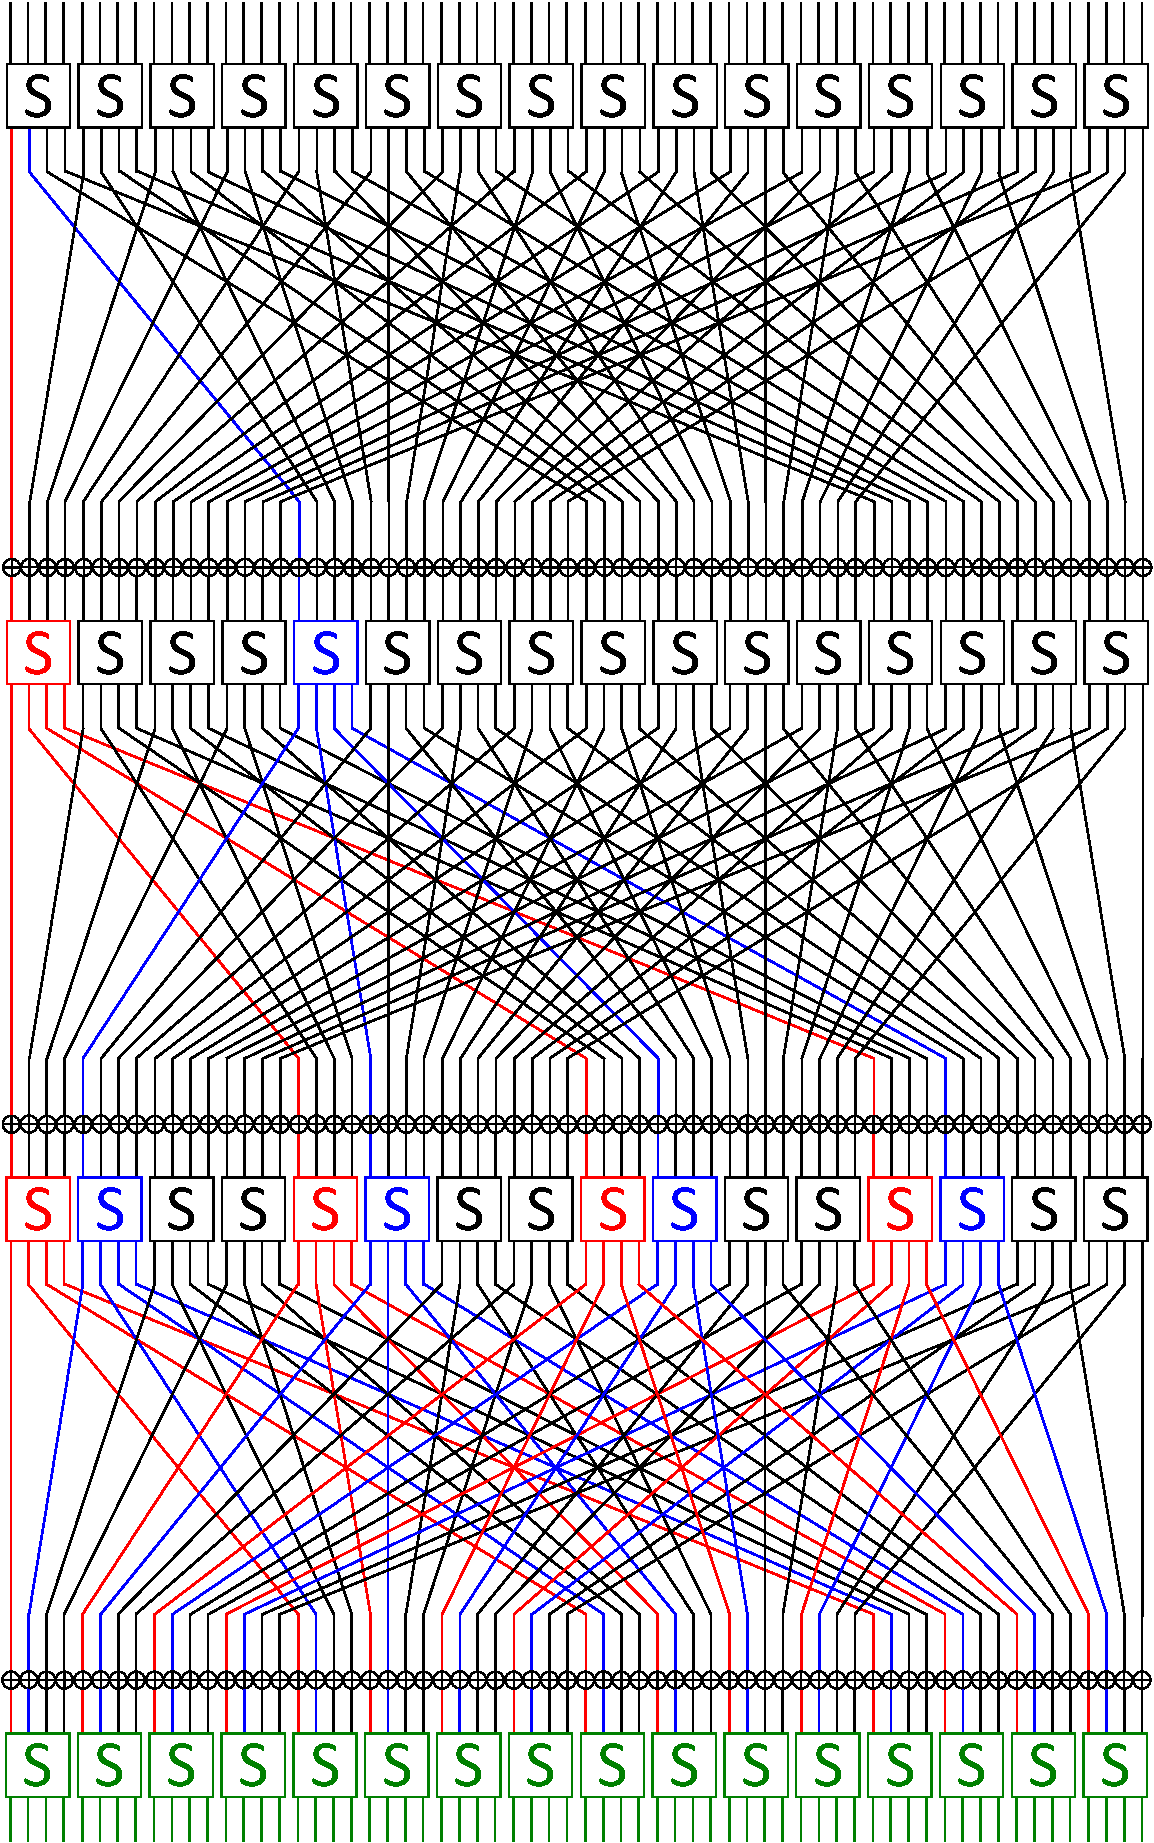
\includegraphics[width=0.8\linewidth]{present_fault_0011}
%     \caption{Fault propagation for the output fault mask $0011$ (Example-2).}
%     \label{example_2}
% \vspace{-0.5cm}
% \end{figure}
% % \end{itemize}

\subsubsection{\textbf{The Generalized Proof}} The above example provide an intuitive explanation for Theorems \ref{th:HW} and \ref{th:Val}. We now present a generalized and formal proof for the same. We present the fault mask characteristics in each of rounds 28, 29, 30 and 31 separately.
\begin{itemize}
\item\textbf{Round 28:} Suppose the adversary injects a fault in nibble $4n+d$, where $n,d\in\{0,1,2,3\}$, and suppose the output fault mask has Hamming weight $x\in\{0,1,\cdots,4\}$. In particular, let $l_1,\cdots,l_{x}\in\{0,1,2,3\}$ be the bits in the output fault mask that are set to 1.
\item\textbf{Round 29:} Consider the effects of the bit $l_1,\cdots,l_x$ in the output fault mask corresponding to nibble $4n+d$ in round 28. As per the generic properties of the diffusion layer of PRESENT discussed in Section \ref{subsec:properties}, these faulty bits will propagate to the nibbles $n+4l_1,\cdots,n+4l_x$ respectively, creating an input fault mask of Hamming Weight 1.

\item \textbf{Round 30:} We now focus on a specific faulty nibble, say nibble $n+4l_1$, in round 29. Once again, as per the generic properties of the diffusion layer of PRESENT discussed in Section \ref{subsec:properties}, the output of this faulty nibble will potentially propagate to the $n^{\text{th}}$ input bit of the nibbles $l_1, l_1+4, l_1+8$ and $l_1+12$ in round 30. Similarly, the output of the faulty nibble $n+l_x$ in round 29 will potentially affect the nibbles $l_x, l_x+4,l_x+8$ and $l_x+12$. \emph{It is important to observe that for each of $l_1,\cdots,l_x$, the set of potentially faulty nibbles in round 30 is disjoint}.

\item \textbf{Round 31:} Finally, we examine the fault propagation to the input of round 31. Consider the faulty quartet of nibbles $l_1, l_1+4, l_1+8$ and $l_1+12$ in round 30. The nibble $l_1$ will potentially spread the fault to the $l^{\text{th}}_1$ input bit of the nibbles $0,4, 8$ and $12$ in round 31. Similarly, the nibble $l_1+4$ will potentially spread the fault to the $l^{\text{th}}_1$ input bit of the nibbles $1,5, 9$ and $13$ in round 31. In general, the faulty nibble $l_{k_1}+4k_2$, where $k_1\in\{1,\cdots,x\}$ and $k_2\in\{0,1,2,3\}$, will potentially spread the fault to the $l^{\text{th}}_{k_1}$ input bit of the nibbles $k_2,k_2+4, k_2+8$ and $k_2+12$ in round 31. This, in turn, implies each nibble in round 31 can receive a faulty input bit from at most $x$ faulty nibbles in round 30. 
\end{itemize}
\noindent Thus, each nibble in round 31 has an input fault mask of Hamming Weight at most $x$. Additionally, since exactly $x$ bits of each input fault mask are 1, and the faulty bits are determined by the values of $l_1,\cdots,l_x$, each input fault mask in round 31 can take $2^x$ values. This completes the proof of Theorems \ref{th:HW} and \ref{th:Val}. 


\subsection{The Key Recovery Process}
\label{subsec:key-recovery}

The fault propagation characteristics described above can now be used to recover multiple key nibbles in parallel. For clarity of presentation, we consider a slightly modified version of PRESENT, where we ignore the bit-permutation operation of round 31. In the absence of the final bit-permutation layer, for any nibble with a non-zero input fault mask, the output is directly XOR-ed with the last round key nibble and output as the ciphertext. Thus, given a correct ciphertext nibble $C$ and a faulty ciphertext nibble $C'$, corresponding to a non-zero input fault mask $\beta$, we have the following differential relation involving the corresponding final round key nibble $K$:
\begin{equation}
S^{-1}\left[C\oplus K\right] \oplus S^{-1}\left[C'\oplus K\right] = \beta\nonumber
\end{equation}
\noindent where $S^{-1}$ denotes the inverse S-Box operation. From the differential uniformity of the PRESENT S-Box, the expected number of values of $K$ satisfying the above equation is one. Now, assuming a non-zero output fault mask with Hamming weight $x$ for the target nibble in round 28, there are $2^x-1$ possible values of the input fault mask $\beta$ in round 31 (this is proven using Theorems \ref{th:HW} and \ref{th:Val}), which in turn gives rise to $2^x-1$ possible differential relations as described above. Hence, any value of $x$ in the set $\{1,2,3\}$ reduces the entropy of the key nibble $K$ by a factor of approximately $2^{4-x}$ on an average, and is hence expected to allow recovering $K$ uniquely after $4/(4-x)$ fault injections (under the assumption that all faults help recover unique key bits). For $x=1,2$ and $3$, the expected number of fault injections are thus $1.33$, $2$ and $4$ respectively. In practice, the required number of fault injections would be slightly higher since the affected key bits would likely overlap; however, key-recovery would still be feasible. On the other hand, for $x=4$, all $15$ possible values of $\beta$ could potentially occur during the attack; hence, \emph{faults with output mask of Hamming weight 4 are not useful for our attack}. 

It is also worth observing that we do not require separate fault injection instances for recovering each key nibble. On the contrary, each fault injection instance in round 28 is expected to yield multiple faulty nibbles in round 31, and each of these nibbles may be analyzed independently and in parallel for key recovery. This inherent parallelism makes the attack very efficient and reduces the overall number of fault injections necessary to recover $64$ bits of the last round key. The attack efficiency is also supported by experimental results in Section \ref{sec:results}. 

The overall attack flow is summarized in Figure~\ref{flow_attack}. Note that the attack can also be repeated in round 27 to additionally recover 64 bits of the penultimate round key, along with 64 bits of the last round key. The combination of two recovered keys can then be used to recover the entire last round key of PRESENT. 

% Like any other side-channel or fault attack on PRESENT, the remaining $16$ bits of the $80$ bit key may be brute-forced even in this attack. An alternative strategy could be to retrieve 64 bits of both the last round key as well as the penultimate round key by repeating the attack twice; once in round 28 and then in round 27. The combination of the two round keys can then be used to recover the entire key of PRESENT. 
%Note that since our proposed DFA is restricted to the data path and does not affect the key-schedule, it is not possible to recover the 16 bits of the last round key that are not combined with the cipher state. Thus, our attack recovers the last round key with an additional brute force complexity of $2^{16}$. 


%\subsection{Summary of the SCA-Aided DFA Procedure}
% \todo[inline]{A figure to show the flow/steps replace textual summary}
% We now present a general summary of the steps in our SCA-aided DFA of PRESENT:
% \begin{itemize}
% \item \textbf{Step-1: Fault Injection.} The adversary executes a correct and faulty instance of the PRESENT encryption with the same plaintext-key pair. In the faulty encryption instance, the adversary injects a single nibble fault in round 28 of PRESENT, and is aware of the precise fault location.
% \item \textbf{Step-2: Side-Channel Analysis.} The adversary now performs a differential analysis of the SCA leakage from round 29 in the correct and faulty computations to identify the output fault mask corresponding to the faulty nibble computation in round 28 (described in Section \ref{subsec:SCA}). f the output fault mask has a Hamming Weight of $4$, the adversary discards the fault injection instance as unexploitable and returns to Step-1. Else, she proceeds to Step-3.
% \item \textbf{Step-3: Analyzing the Fault Propagation.} Using the analysis methodology enumerated in Section \ref{subsec:propagation}, the adversary identifies the $2^x-1$ possible non-zero input fault masks for each nibble in round 31.
% \item \textbf{Step-4: Recovering the Key Nibbles.} For each faulty nibble in the final ciphertext, the adversary performs the analysis described in Section \ref{subsec:key-recovery} to refine the potential values for the corresponding final-round key nibble. 
% \end{itemize}
% \noindent The above steps are repeated till the adversary uniquely identifies each of the $16$ nibbles of the final round key for the modified PRESENT. Finally, she applies the inverse bit-permutation of PRESENT to this recovered key and obtains the last round key of the original PRESENT.


\tikzstyle{decision} = [diamond, draw, fill=blue!20, 
    text width=7.5em, text badly centered, node distance=3cm, inner sep=0pt]
\tikzstyle{block} = [rectangle, draw, fill=blue!20, 
    text width=8em, text centered, rounded corners, minimum height=4em]
\tikzstyle{gblock} = [rectangle, draw, fill=green!20, 
    text width=8em, text centered, rounded corners, minimum height=4em]
\tikzstyle{line} = [draw, -latex']
\tikzstyle{eline} = [draw, -]
\tikzstyle{cloud} = [draw, ellipse,fill=red!20, node distance=3cm,
    minimum height=2em]
\tikzstyle{decision answer}=[near start,color=black]
\tikzstyle{coord}=[coordinate, node distance=6mm and 25mm]

\begin{figure}
\centering
\begin{tikzpicture}[node distance = 2cm, auto, scale=0.6, every node/.style={scale=0.65}]
	
	\node [block] (corr) {correct encryption};
	\node [cloud, right of=corr, node distance=4cm] (ctrace) {correct trace};
    \node [block, below of=corr] (fa) {faulty encryption};
	\node [cloud, right of=fa, node distance=4cm] (ftrace) {faulty trace};
    \node [block, below of=fa] (sca) {side-channel analysis};
    \node [block, below of=sca] (propagation) {analyze fault propagation};
	\node [cloud, right of=propagation, node distance=4cm] (fmask) {fault mask};
	\node [coord, left of=propagation, node distance=3cm] (onemore) {};
    \node [decision, below of=propagation] (decide) {is hamming weight 4?};
    \node [block, below of=decide, node distance=3cm] (recover) {combined analysis};
	\node [cloud, above right = 0.1cm and 1cm of recover] (ctext) {correct ciphertext};
	\node [cloud, right of=recover, node distance=4cm] (fmask2) {fault mask};
	\node [cloud, below right = 0.1cm and 1cm of recover] (ftext) {faulty ciphertext};
	\node [decision, below of=recover] (isdone) {are all 16 nibbles recovered?};
	\node [gblock, below of=isdone, node distance=3cm] (done) {attack successful};

	\path [line] (corr) -- (fa);
	\path [line, dashed] (corr) -- (ctrace);
    \path [line] (fa) -- (sca);
	\path [line, dashed] (fa) -- (ftrace);
    \path [line] (sca) -- (propagation);
	\path [line, dashed] (propagation) -- (fmask);
    \path [line] (propagation) -- (decide);
    \path [eline](decide) -| node [near start] {yes} (onemore);
    \path [line] (onemore) |- (fa);
    \path [line] (decide) -- node [decision answer]{no}(recover);
	\path [line] (recover) -- (isdone);
	\path [line, dashed] (ctext) -- (recover);
	\path [line, dashed] (ftext) -- (recover);
	\path [line, dashed] (fmask2) -- (recover);
	\path [eline] (isdone) -| node [near start] {no} (onemore);
	\path [line] (isdone) -- node {yes}(done);
\end{tikzpicture}
\caption{Execution steps for Proposed Combined Attack}
\label{flow_attack}
\vspace{-0.5cm}
\end{figure}


\section{Experimental Results}
\label{sec:results}
\subsection{The Combined SCA+FA Setup}

The setup for our combined SCA and DFA-based attack is depicted in Figure~\ref{setup}. The core of the setup consists of near-infrared diode pulse laser (1064 nm wavelength) with the maximum output power of 20 W. 
This power is further reduced to $\approx$ 8 W with usage of 20$\times$ objective lens that scales the effective spot size to $15\times3.5 \mu m$. 
The laser activation length was set to 150 ns and the laser power was set to 3\%, resulting to $\approx$ 0.24 W.
\begin{figure}
	\centering
	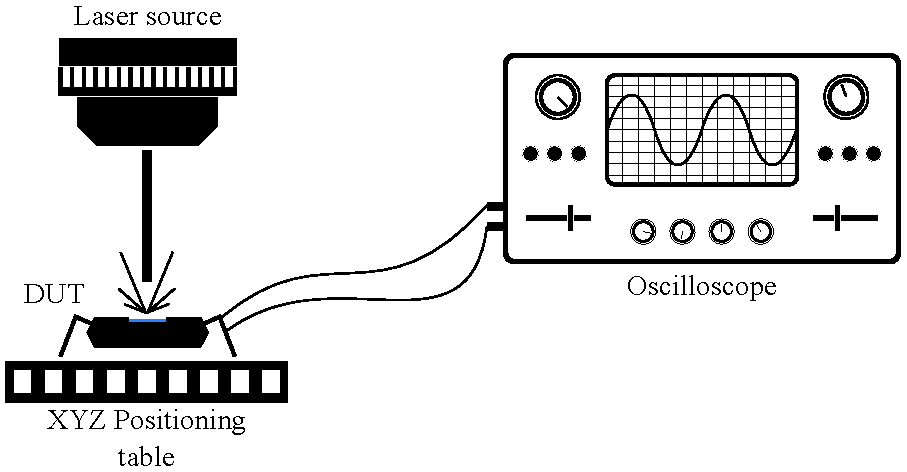
\includegraphics[width=0.8\linewidth]{combined_setup}
    \caption{Experimental setup for the SCA-aided DFA procedure.}
    \label{setup}
\end{figure}

As the device under test (DUT), we used ATmega328P microcontroller, decapsulated from the back-side and mounted on Arduino UNO development board. The area of the chip is $3\times 3~mm^2$, while the sensitive area covers $\approx$ 0.05\% of the whole chip size. The implementation of PRESENT we used computes the addRoundKey byte-wise and S-Box nibble-wise, therefore, we had to take this into account during the fault model estimation.
The attack has to be likewise adjusted if the S-Box is computed byte-wise.

To control the impact location, we used XYZ positioning table with the spatial precision of 0.05 $\mu m$.
Timing precision is achieved by inserting the trigger at the start of round 28.

For the side-channel leakage measurement, we used a digital oscilloscope, capturing the time frame of one round after the fault was injected. In order to distinguish the fault mask, we first profiled the standard power consumption by calculating an average of 100 encryptions. As the repeatability of the fault was 100\%, another 100 experiments were done while injecting the fault at the same position and same timing and again, averaging these traces. Afterwards, we calculated a difference of these two traces and it gave us the knowledge of the injected fault mask in the previous round. 


We would like to point out that both the triggering for fault injection and the averaging of the power traces are optional. By observing the side-channel trace in our case, it was straightforward to pin-point beginning and ending of each round and each operation (S-BoxLayer, pLayer, addRoundKey) had a unique side-channel signature (this can be seen in the upper part of Figure~\ref{3rounds}). Similarly, the 
fault mask was recoverable from single trace. Indeed, if the repeatability of the fault is low, averaging will be difficult.

\subsection{Determination of Fault Mask}

In the following, we will detail the process of estimating the fault mask, based on laser fault injection parameters, and side-channel leakage.

\begin{figure}
	\centering
	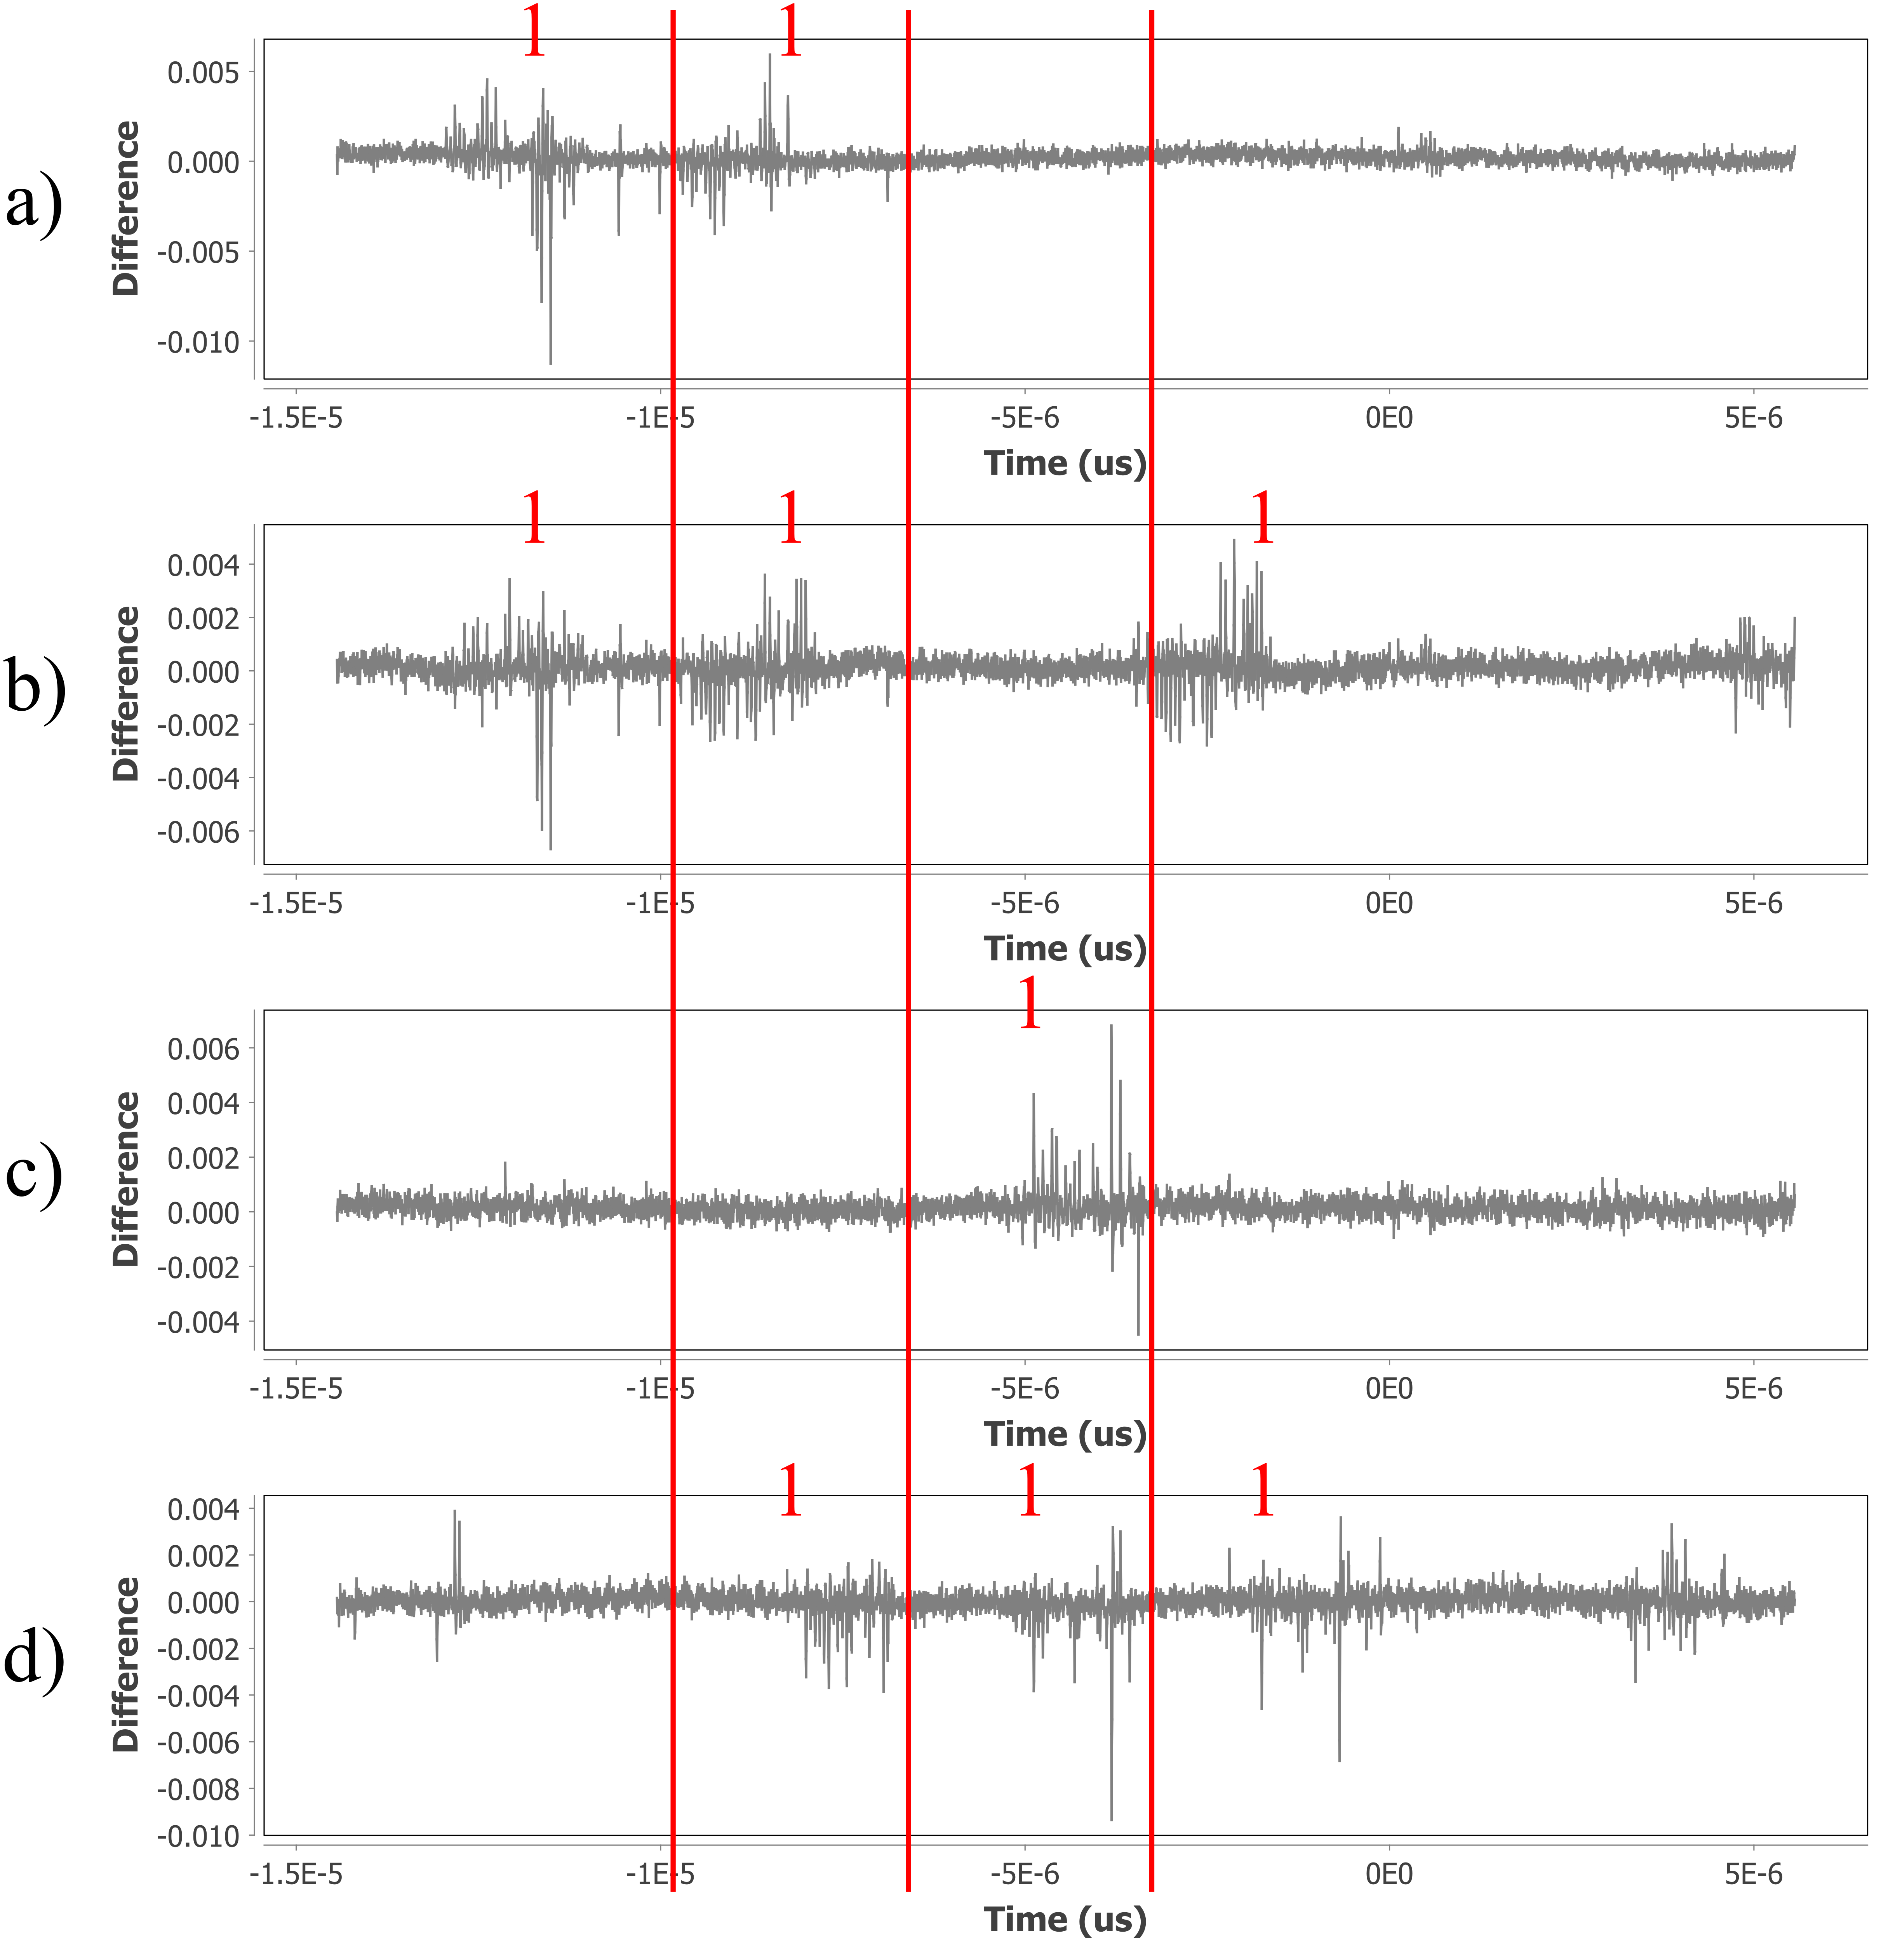
\includegraphics[width=0.8\linewidth]{sca_masks1}
    \caption{Fault mask determination from SCA leakage.}
    \label{sca_masks}
\end{figure}

\begin{table}
\centering
\caption{Analysis of the leakage difference patterns from Figure~\ref{sca_masks}.}
\label{sca_masks_analysis}
\begin{tabular}{c r c c}
\textbf{Trace} & \textbf{Offset (ns)} & \textbf{I/P Fault Mask:R29} & \textbf{O/P Fault Mask:R28} \\ \hline
a) & 4032 & 0000000000800080 & 00000000000C0000 \\
b) & 4914 & 0040000000400040 & 0000000000D00000 \\
c) & 7686 & 0000080000000000 & 0000000200000000 \\
d) & 9072 & 0200020002000000 & 0000070000000000 \\
%e) & 10143 & 0100010001000000 & 0000700000000000 \\
%f) & 10773 & 0000800000000000 & 0002000000000000 \\
\hline
\end{tabular}
\vspace{-0.3cm}
\end{table}

There are two steps of determining the faulty nibble and the mask in round 28:
\begin{enumerate}
	\item In order to get the information on which nibble has been faulted, we have to check the timing from the trigger. The S-Box computation on the DUT takes $\approx 11 \mu s$. During the profiling phase, the timing for processing each nibble can be estimated with 100\% success rate. Nibbles are processed in a reversed order (15 to 0), therefore, for example, w.r.t defined trigger signal, nibble 14 starts with a timing offset of $2,331$ ns, while nibble 0 starts at $12,537$ ns.
    %\todo[inline]{If the min time for an S-Box is 11 $\mu$ sec, how can the 14th S-Box start at 2331 ns? Pls chk.}
    \item For estimating the fault mask, we have to check the side-channel leakage in the round 29. This process is depicted in Figure~\ref{sca_masks} and the values corresponding to each power trace are detailed in Table~\ref{sca_masks_analysis}. As can be easily seen, the difference trace shows the nibble position in round 29 which has a different value from the trace corresponding to non-faulty execution. This position can be easily determined from the profiling phase and comparing different traces. Reverse engineering techniques can also be applied in this case to determine the round and nibble position. In Figure~\ref{sca_masks}, the red guiding lines show the relative position of nibbles, while `1' indicates that there is a difference w.r.t. the original trace. Then, by applying a reverse bit-permutation, the output S-Box difference of round 28 can be determined.
\end{enumerate}

\subsection{Key Recovery: Performance and Efficiency}

We now present results illustrating the number of necessary fault injections to recover the last round key of PRESENT using the faults. Our SCA experiments demonstrated that nearly all the output fault masks obtained upon fault injection had Hamming weights of $1$, $2$ and $3$, which is precisely the useful class of faults for our attack. Figure \ref{plot:prop} presents a comparison of the estimated number of fault injections required under each kind of fault mask for fault propagation to a given number of nibbles in the ciphertext. Recall that the DFA can recover a given key nibble only if the fault propagates to that nibble in the last round. Hence, the efficiency of the attack depends on the average number of fault injections required for the fault to propagate to each nibble. Quite intuitively, greater the Hamming weight of the output fault mask in the target round, the faster the fault propagates to a larger number of nibbles in the subsequent rounds. This is also reflected in our experimental results. However, a higher Hamming weight of the fault mask also reduces exploitation potential due to enhanced fault propagation in rounds 29 and 30, as illustrated next.

We now present the average number of fault injections required to recover a given number of nibbles of the last round key for each category of fault mask in Figure \ref{plot:recover}. Quite evidently, key recovery for fault masks with Hamming weights 1 and 2 requires a significantly lesser number of fault injections than with Hamming weight 3. This is in accordance with the theoretical estimate for the required number of fault injections in Section \ref{subsec:key-recovery}. On average, a combination of fault masks with Hamming Weights 1 and 2 recovers 64 bits of the key in \textbf{7-8 fault injections}, which is at par with the best known fault attack on PRESENT, while the best case scenario allows recovering 64 bits of the key with \textbf{$4$ fault injections}. The best case scenario is typically encountered when using fault masks of Hamming weight $1$, and the fault diffuses to all nibbles of the final round in each injection. The worst case scenario, on the other hand, is encountered with fault masks of Hamming weight $3$, when $19$ fault injections are found to be necessary for key recovery.
\begin{figure}[t]
% \captionsetup{font=scriptsize}
\centering
%\begin{tabular}{cc}
% \begin{subfigure}{0.5\textwidth}
% \captionsetup{font=scriptsize}
% \centering
% \hspace*{-10mm}
% \subfloat[\scriptsize{Search Time v/s Number of Documents (Actual)}]{
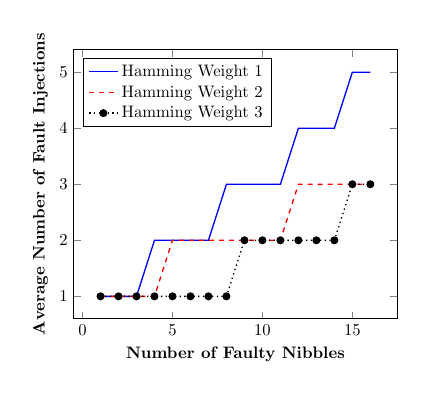
\begin{tikzpicture}[scale = 0.6]
	 \begin{axis}[
	 		xlabel= \textbf{Number of Faulty Nibbles},
	 		ylabel= \textbf{Average Number of Fault Injections},
	 		legend pos={north west}
	 		]
% 	 
	 \addplot[blue,thick] plot coordinates{
	 	(1, 1)
		(2, 1)
		(3, 1)
		(4, 2)
		(5, 2)
		(6, 2)
		(7, 2)
		(8, 3)
		(9, 3)
		(10, 3)
        (11, 3)
		(12, 4)
		(13, 4)
		(14, 4)
		(15, 5)
		(16, 5)
	 };\addlegendentry{Hamming Weight 1}
     
     \addplot[red,dashed,thick] plot coordinates{
	 	(1, 1)
		(2, 1)
		(3, 1)
		(4, 1)
		(5, 2)
		(6, 2)
		(7, 2)
		(8, 2)
		(9, 2)
		(10, 2)
        (11, 2)
		(12, 3)
		(13, 3)
		(14, 3)
		(15, 3)
		(16, 3)
	 };\addlegendentry{Hamming Weight 2}
     
      \addplot[black, thick, dotted, mark=*, mark options={solid}] plot coordinates{
	 	(1, 1)
		(2, 1)
		(3, 1)
		(4, 1)
		(5, 1)
		(6, 1)
		(7, 1)
		(8, 1)
		(9, 2)
		(10, 2)
        (11, 2)
		(12, 2)
		(13, 2)
		(14, 2)
		(15, 3)
		(16, 3)
	 };\addlegendentry{Hamming Weight 3}
\end{axis}
\end{tikzpicture}
\caption{Fault Propagation: Average Number of Fault Injections v/s Number of Faulty Nibbles}
\label{plot:prop}
 %\vspace*{-6mm}
\end{figure}

\begin{figure}[t]
% \captionsetup{font=scriptsize}
\centering
% \begin{subfigure}{0.5\textwidth}
% \captionsetup{font=scriptsize}
%\centering
% \hspace*{-10mm}
% \subfloat[\scriptsize{Search Time v/s Number of Documents (Actual)}]{
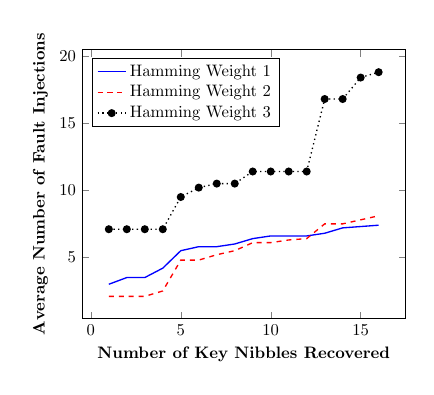
\begin{tikzpicture}[scale = 0.6]
	 \begin{axis}[
	 		xlabel= \textbf{Number of Key Nibbles Recovered},
	 		ylabel= \textbf{Average Number of Fault Injections},
	 		legend pos={north west}
	 		]
% 	 
	 \addplot[blue,thick] plot coordinates{
	 	(1, 3)
		(2, 3.5)
		(3, 3.5)
		(4, 4.2)
		(5, 5.5)
		(6, 5.8)
		(7, 5.8)
		(8, 6.0)
		(9, 6.4)
		(10, 6.6)
        (11, 6.6)
		(12, 6.6)
		(13, 6.8)
		(14, 7.2)
		(15, 7.3)
		(16, 7.4)
	 };
     \addlegendentry{Hamming Weight 1}  
     
     \addplot[red,thick, dashed] plot coordinates{
	 	(1, 2.1)
		(2, 2.1)
		(3, 2.1)
		(4, 2.5)
		(5, 4.8)
		(6, 4.8)
		(7, 5.2)
		(8, 5.5)
		(9, 6.1)
		(10, 6.1)
        (11, 6.3)
		(12, 6.4)
		(13, 7.5)
		(14, 7.5)
		(15, 7.8)
		(16, 8.1)
	 };
     \addlegendentry{Hamming Weight 2}
     
      \addplot[black,thick,dotted, mark=*, mark options={solid}] plot coordinates{
	 	(1, 7.1)
		(2, 7.1)
		(3, 7.1)
		(4, 7.1)
		(5, 9.5)
		(6, 10.2)
		(7, 10.5)
		(8, 10.5)
		(9, 11.4)
		(10, 11.4)
        (11, 11.4)
		(12, 11.4)
		(13, 16.8)
		(14, 16.8)
		(15, 18.4)
		(16, 18.8)
	 };
     \addlegendentry{Hamming Weight 3}
\end{axis}
\end{tikzpicture}
\caption{Key Recovery: Average Number of Fault Injections v/s Number of Key Nibbles Recovered}
\label{plot:recover}
%\vspace*{-4mm}
\end{figure}

\subsection{Applicability to Hardware Implementations}

A final point to note is that although we experimentally demonstrate our attack on a software implementation of PRESENT, the attack is also applicable on hardware (HW) implementations.
Low-cost nibble HW implementations will have the same vulnerability.
Parallel implementations will be harder to exploit, nevertheless, localized measurements can be used to recover the fault mask and perform the attack.
%For a hardware implementation processing the nibbles in a parallel fashion, the attacker would need side-channel equipment with localized measurement capability to recover the fault mask. Once the fault mask is recovered, the same attack follows. 

\section{Discussion}
\subsection{Extension to Other Rounds}
While it is relatively easy to determine the faulty nibbles in round 29, this process becomes harder once the propagation of the fault produces collisions. For example, let us assume that after several rounds, the difference reaches nibbles 8 and 11, producing the S-Box output masks of value `8' for both nibbles. These two bits will propagate to nibble 15 in the next round, producing the S-Box input mask `C'. Such a difference cannot be easily seen from the power trace by just observing the differential peaks, and therefore, we can only assume that some of the nibbles between 8-11 in the previous round were faulted. This behavior would require creation of SCA templates for each nibble and each fault mask, resulting in total of 256 different templates.   

Similar scenario can be seen in Figure~\ref{3rounds}, depicting the last three rounds of encryption -- upper part is the power trace of the non-faulty encryption process, so that it makes it possible to estimate particular rounds. Lower part is the differential trace which shows that while it is trivial to determine the fault mask for round 28 based on difference in round 29, following rounds are hard to analyze.
\begin{figure}
	\centering
	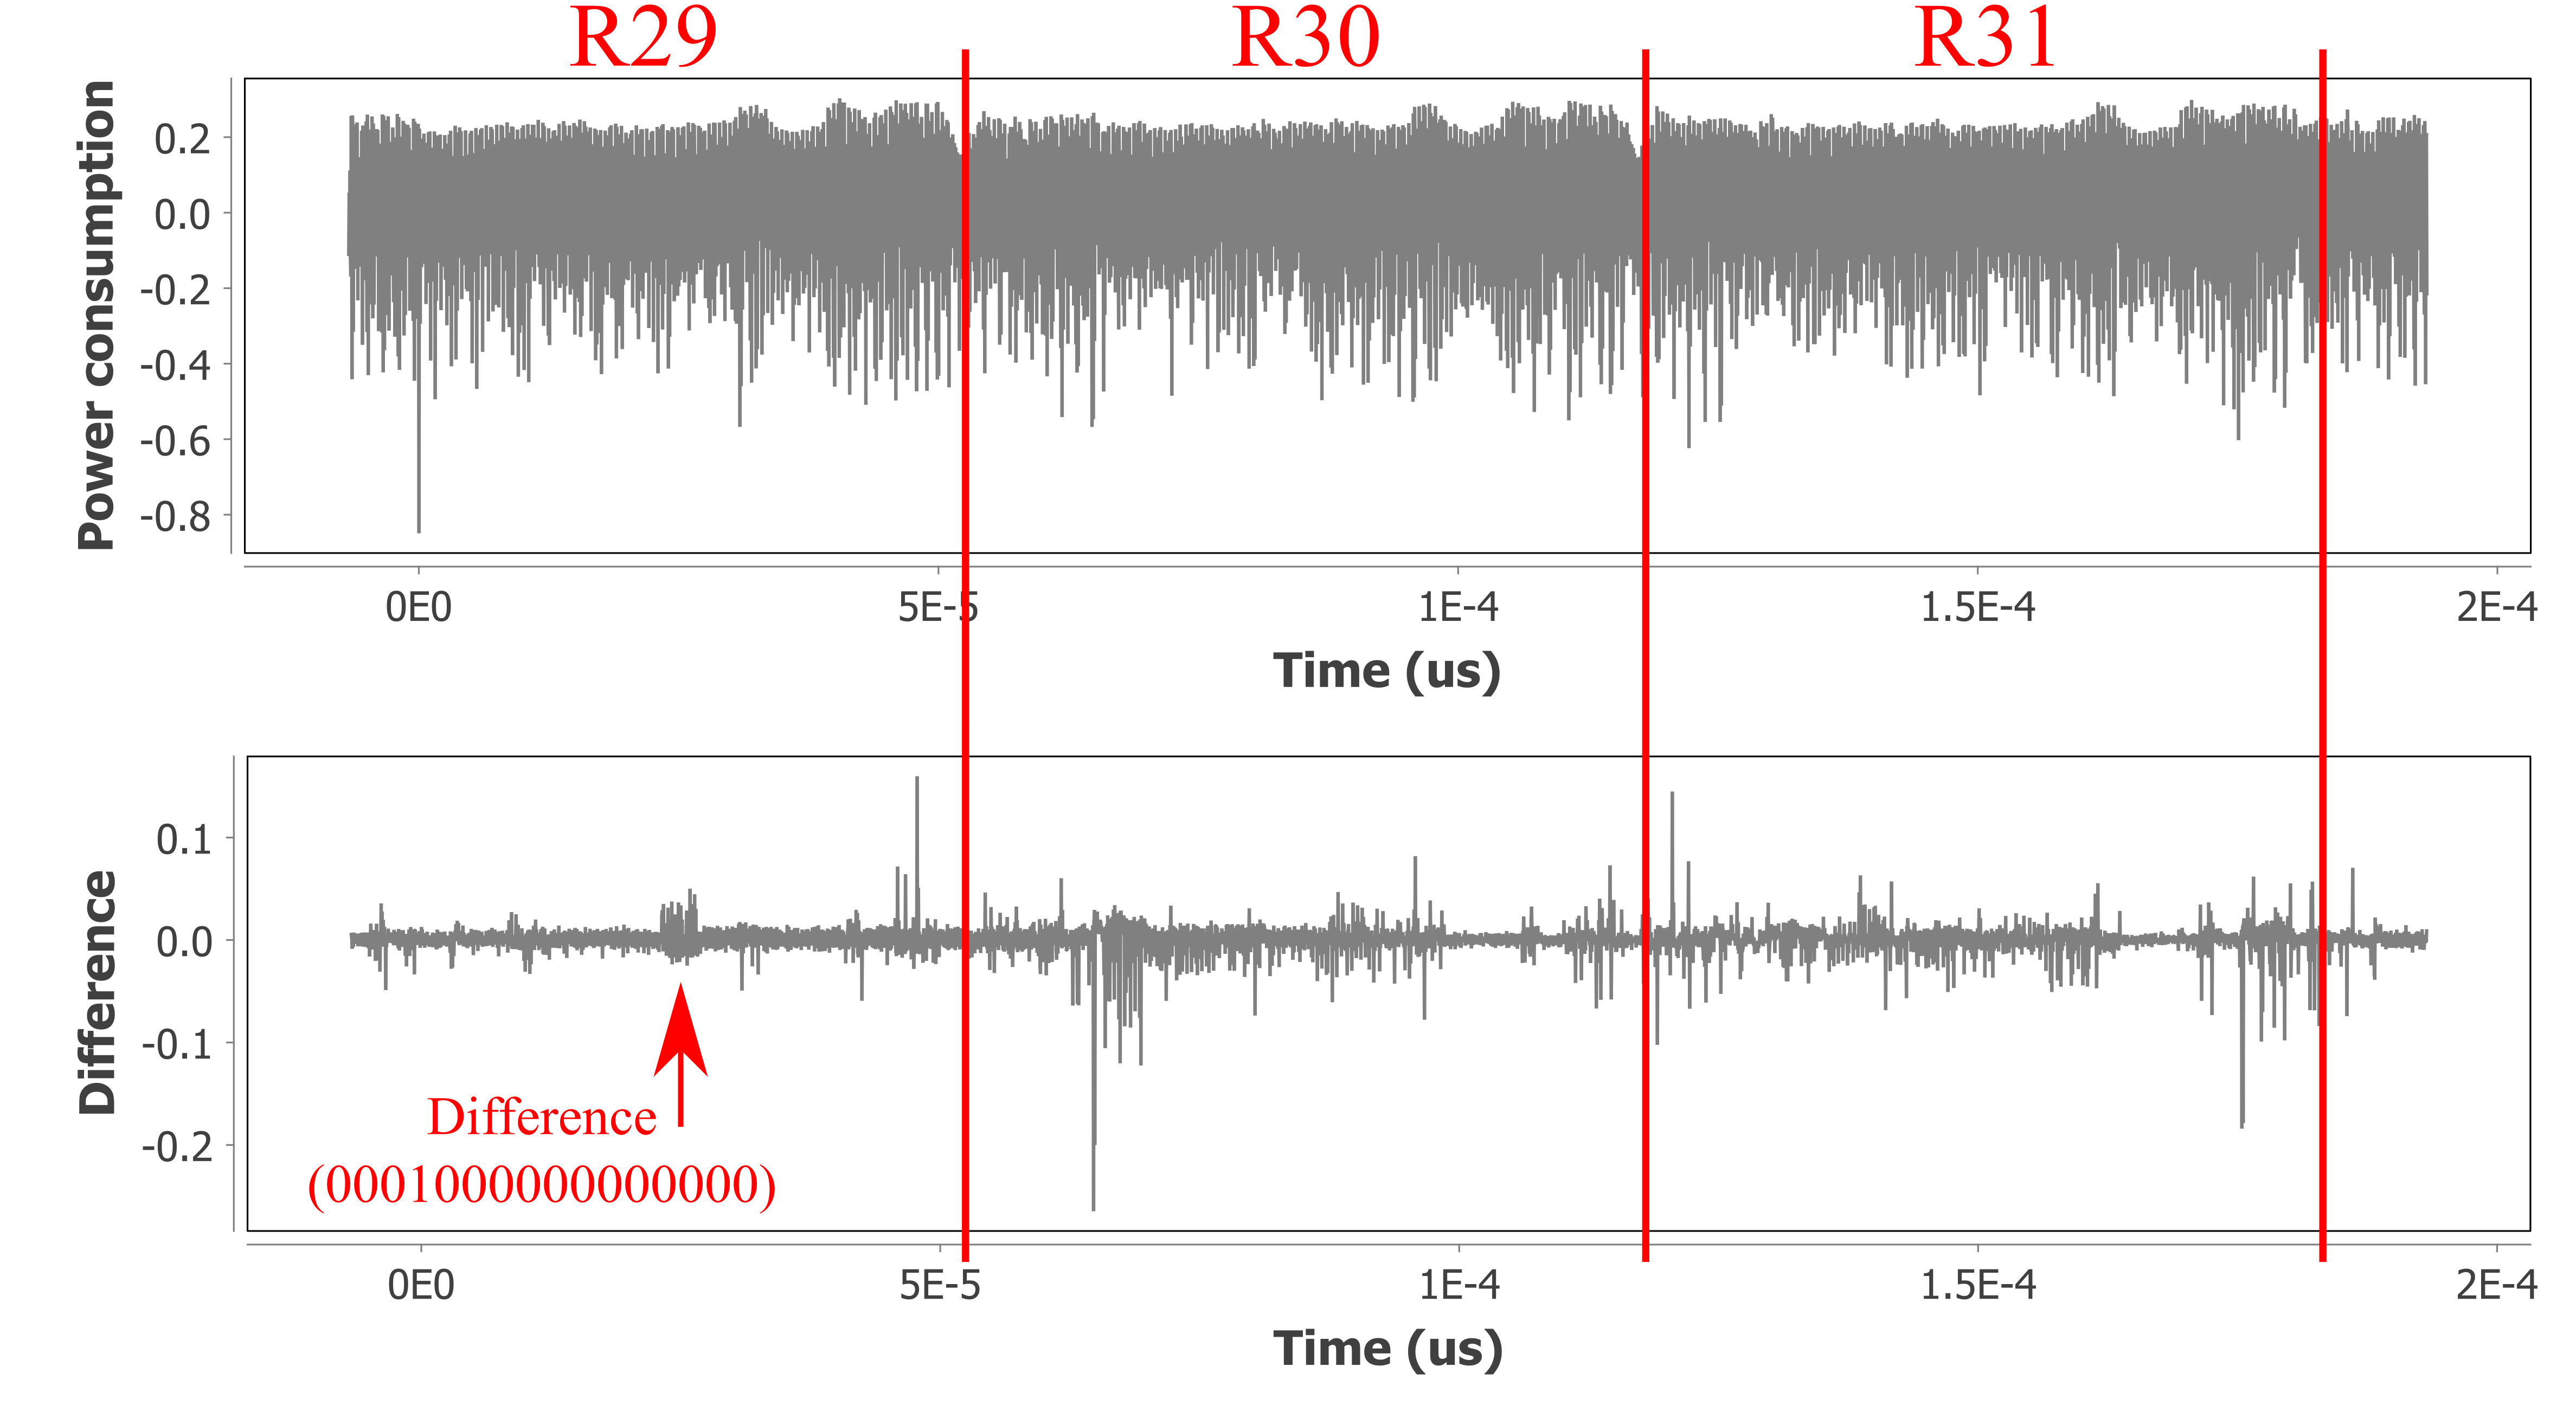
\includegraphics[width=0.9\linewidth]{3rounds_difference}
    \caption{Power trace for the last three rounds with a corresponding differential trace.}
    \label{3rounds}
   % \vspace{-0.4cm}
\end{figure}


\subsection{Extension to Other PRESENT-like Block Ciphers}

The combined SCA and FA based attack on PRESENT can also be extended to other PRESENT-like block ciphers that use bit-permutations for diffusion. One such recently proposed block cipher is GIFT \cite{gift}. GIFT has two versions - GIFT-64 with a 64 bit plaintext block and GIFT-128 with a 128 bit plaintext block. The bit-permutation layer for GIFT-64 differs from PRESENT, which lends it some additional advantages against cryptanalytic attacks and better efficiency in software. However, similar to PRESENT, the bit-permutation layer of GIFT-64 also ensures that each of the four sets of nibbles, namely [0-4],[5-8], [6-11] and [12-15] affect exactly four non-overlapping sets of nibbles $\{0,4,8,12\}$, $\{1,5,9,13\}$, $\{2,6,10,14\}$ and $\{3,7,11,15\}$, respectively. Since it is this property of the bit-permutation that our combined attack exploits, the attack is also applicable to GIFT-64 with the same efficiency as PRESENT. An extension of the attack is also applicable in case of GIFT-128, although a detailed description of the same is beyond the scope of the current paper. 

\emph{It is, however, interesting to see that the combined attack methodology would fail against ciphers such as AES or LED that use MDS layers.} The diffusion characteristics of an MDS layer would break any correlation between the output fault mask of a prior round and the eventual input fault mask at a later round, by causing the fault to always diffuse to the maximum possible number of nibbles in each round. 

% To the best of our knowledge, no prior fault attack has shed light on this apparently inherent vulnerability of bit-permutation based diffusion layers towards combined attacks. 

% This leads to the following interesting observation: \emph{While bit-permutations are a popular choice for lightweight block ciphers owing to their greater efficiency in hardware as compared to MDS layers, they are prone to a class of combined SCA+FA attacks that MDS layers resist}. To the best of our knowledge, no prior fault attack has shed light on this apparently inherent vulnerability of bit-permutation based diffusion layers towards combined attacks. 

% A possible future work is to compare and contrast the vulnerability of MDS layers and bit-permutations against a wider class of fault attacks in general.

\subsection{Possible Countermeasures}

We briefly discuss potential countermeasures and their effectiveness in resisting our combined attack methodology on bit-permutation based SPN block ciphers. Standard fault detection mechanisms such as spatial and temporal redundancy could potentially increase the number of fault injections required; but they can be bypassed using biased fault injection techniques \cite{patranabis2015biased} that allow injecting the same fault in both the original and redundant computations with high probability. Standard side-channel countermeasures such as masking could be incorporated to make the attack more difficult in the sense that one might require higher order analysis over a larger number of power traces to retrieve the desired fault mask value in such a scenario. Other less costly alternatives to masking such as shuffling and hiding might also increase the complexity of retrieving the fault mask. 

% It would be an interesting future work to investigate the exact security afforded by the presence of SCA countermeasures against our attack. 



\section{Conclusion}

In this paper, we have practically demonstrated the strength of combining SCA and FA in attacking PRESENT-like block ciphers that use bit-permutations instead of MDS layers for diffusion. We used a laser fault injection based setup to inject nibble faults in the ${28}^{\text{th}}$ round of PRESENT, and perform a simplified variant of differential power analysis on the correct and faulty execution trace to fully infer the resulting fault mask. We subsequently demonstrated a generalized DFA expanding across the last four rounds of PRESENT that allows reducing the entropy of the input fault masks for the last round, and recovering multiple key nibbles in parallel. We have practically corroborated our theoretical observations via actual fault injection and key recovery attacks on an ATmega328P microcontroller-based implementation of PRESENT-80. Our attack exposes an interesting and unexplored vulnerability of PRESENT-like block ciphers that use bit-permutations as opposed to MDS layers for diffusion. Further research can look into vulnerability of MDS matrix-based linear layer for similar attacks. Extension of these attacks on protected targets can also be an interesting line of work.

% that while bit-permutations are a popular choice for lightweight block ciphers owing to their greater efficiency in hardware as compared to MDS layers, they are prone to a class of combined SCA+FA attacks that MDS layers resist.

% An interesting future scope of research is to investigate the effect of side-channel countermeasures on the proposed combination of SCA and FA in this paper.

\bibliographystyle{IEEEtran}
\bibliography{comb}
\end{document}

